\documentclass[11pt]{article}
\usepackage[margin=0.8in]{geometry}
\usepackage{amsmath,amssymb}
\usepackage{tikz}
\usepackage{hyperref}
\usepackage{enumitem}
\setlength{\parindent}{0pt}
\setlength{\parskip}{6pt}
\hypersetup{colorlinks=true,urlcolor=blue,linkcolor=black}
\begin{document}
\title{GED Math Template Bank\\\large Questions, Answer Rules, and Examples}
\author{Math Tutor Website}
\date{October 4, 2026}
\maketitle
163 original template families, mapped to 62 content indicators. This is a practice bank, not an official GED publication or a guarantee of exhaustive exam coverage.
Reusable LaTeX strings, variable ranges, and machine-readable answer rules are in the accompanying JSON and Markdown files. This document includes reusable template source and one rendered example per family. Numeric-form compatibility depends on the listed engine features.
\textbf{Grading:} Exact rational arithmetic by default. Rounding is accepted only when the question requests it, using ROUND\_HALF\_UP. For circle and solid questions, use the stated value $\pi=3.14$. Symbolic answers require domain-aware equivalence checks; factoring also requires factored structure.
\textbf{Access:} Students must log in and receive an administrator assignment for each practice set. Freeze generated questions and answers per attempt; preserve all attempt results.
\textbf{Sources:} \href{https://www.ged.com/content/dam/websites/ged/resources/en/assessment-guide-for-educators-math.pdf}{GED assessment guide}; \href{https://www.ged.com/content/dam/websites/ged/post/math-formula-sheet.pdf}{GED formula sheet}. Questions and explanations in this bank are newly authored.
\tableofcontents
\newpage
\section{Number sense and arithmetic}
\subsection{N01 -- Integer addition}
\textbf{Targets:} Q.2.a\quad\textbf{Mode:} numeric
\textbf{Question:} Compute \(-9+(7)\).
\textbf{Answer:} \(-2\)
\textbf{Method:} Add the signed values.
\textbf{Reusable LaTeX template:}
\begin{verbatim}
Compute \({a:-30–30}+({b:-30–30})\).
\end{verbatim}
\textbf{Answer formula/rule:}
\begin{verbatim}
a+b
\end{verbatim}
\textbf{Generation ranges:} a: -30 to 30; b: -30 to 30
\medskip\hrule\medskip
\subsection{N02 -- Integer subtraction}
\textbf{Targets:} Q.2.a\quad\textbf{Mode:} numeric
\textbf{Question:} Compute \(-27-(12)\).
\textbf{Answer:} \(-39\)
\textbf{Method:} Subtracting a number is adding its opposite.
\textbf{Reusable LaTeX template:}
\begin{verbatim}
Compute \({a:-30–30}-({b:-30–30})\).
\end{verbatim}
\textbf{Answer formula/rule:}
\begin{verbatim}
a-b
\end{verbatim}
\textbf{Generation ranges:} a: -30 to 30; b: -30 to 30
\medskip\hrule\medskip
\subsection{N03 -- Integer multiplication}
\textbf{Targets:} Q.2.a\quad\textbf{Mode:} numeric
\textbf{Question:} Compute \((-4)\times(8)\).
\textbf{Answer:} \(-32\)
\textbf{Method:} Multiply magnitudes and apply the sign rule.
\textbf{Reusable LaTeX template:}
\begin{verbatim}
Compute \(({a:-12–12})\times({b:-12–12})\).
\end{verbatim}
\textbf{Answer formula/rule:}
\begin{verbatim}
a*b
\end{verbatim}
\textbf{Generation ranges:} a: -12 to 12; b: -12 to 12
\medskip\hrule\medskip
\subsection{N04 -- Integer division}
\textbf{Targets:} Q.2.a\quad\textbf{Mode:} numeric
\textbf{Question:} Compute \(-49\div 3\).
\textbf{Answer:} \(\frac{-49}{3}\)
\textbf{Method:} Write the quotient as a reduced fraction if necessary.
\textbf{Reusable LaTeX template:}
\begin{verbatim}
Compute \({a:-100–100}\div {b:1–12}\).
\end{verbatim}
\textbf{Answer formula/rule:}
\begin{verbatim}
a/b
\end{verbatim}
\textbf{Generation ranges:} a: -100 to 100; b: 1 to 12
\medskip\hrule\medskip
\subsection{N05 -- Fraction addition}
\textbf{Targets:} Q.2.a\quad\textbf{Mode:} numeric
\textbf{Question:} Compute \(\frac{7}{9} + \frac{2}{2}\).
\textbf{Answer:} \(\frac{16}{9}\)
\textbf{Method:} Use fraction arithmetic and reduce the result.
\textbf{Reusable LaTeX template:}
\begin{verbatim}
Compute \(\frac{{a:1–12}}{{b:2–12}} + \frac{{c:1–12}}{{d:2–12}}\).
\end{verbatim}
\textbf{Answer formula/rule:}
\begin{verbatim}
a/b + c/d
\end{verbatim}
\textbf{Generation ranges:} a: 1 to 12; b: 2 to 12; c: 1 to 12; d: 2 to 12
\medskip\hrule\medskip
\subsection{N06 -- Fraction subtraction}
\textbf{Targets:} Q.2.a\quad\textbf{Mode:} numeric
\textbf{Question:} Compute \(\frac{2}{3} - \frac{1}{4}\).
\textbf{Answer:} \(\frac{5}{12}\)
\textbf{Method:} Use fraction arithmetic and reduce the result.
\textbf{Reusable LaTeX template:}
\begin{verbatim}
Compute \(\frac{{a:1–12}}{{b:2–12}} - \frac{{c:1–12}}{{d:2–12}}\).
\end{verbatim}
\textbf{Answer formula/rule:}
\begin{verbatim}
a/b - c/d
\end{verbatim}
\textbf{Generation ranges:} a: 1 to 12; b: 2 to 12; c: 1 to 12; d: 2 to 12
\medskip\hrule\medskip
\subsection{N07 -- Fraction multiplication}
\textbf{Targets:} Q.2.a\quad\textbf{Mode:} numeric
\textbf{Question:} Compute \(\frac{2}{5} \times \frac{9}{6}\).
\textbf{Answer:} \(0.6\)
\textbf{Method:} Use fraction arithmetic and reduce the result.
\textbf{Reusable LaTeX template:}
\begin{verbatim}
Compute \(\frac{{a:1–12}}{{b:2–12}} \times \frac{{c:1–12}}{{d:2–12}}\).
\end{verbatim}
\textbf{Answer formula/rule:}
\begin{verbatim}
a/b * c/d
\end{verbatim}
\textbf{Generation ranges:} a: 1 to 12; b: 2 to 12; c: 1 to 12; d: 2 to 12
\medskip\hrule\medskip
\subsection{N08 -- Fraction division}
\textbf{Targets:} Q.2.a\quad\textbf{Mode:} numeric
\textbf{Question:} Compute \(\frac{12}{9}\div\frac{11}{10}\).
\textbf{Answer:} \(\frac{40}{33}\)
\textbf{Method:} Multiply the first fraction by the reciprocal of the second.
\textbf{Reusable LaTeX template:}
\begin{verbatim}
Compute \(\frac{{a:1–12}}{{b:2–12}}\div\frac{{c:1–12}}{{d:2–12}}\).
\end{verbatim}
\textbf{Answer formula/rule:}
\begin{verbatim}
(a/b)/(c/d)
\end{verbatim}
\textbf{Generation ranges:} a: 1 to 12; b: 2 to 12; c: 1 to 12; d: 2 to 12
\medskip\hrule\medskip
\subsection{N09 -- Decimal addition}
\textbf{Targets:} Q.2.a\quad\textbf{Mode:} numeric
\textbf{Question:} Compute \(4.9 + 9.5\).
\textbf{Answer:} \(14.4\)
\textbf{Method:} Treat the decimals as exact fractions, then calculate.
\textbf{Reusable LaTeX template:}
\begin{verbatim}
Compute \({a} + {b}\).
\end{verbatim}
\textbf{Answer formula/rule:}
\begin{verbatim}
a + b
\end{verbatim}
\textbf{Generation ranges:} u: 11 to 99; v: 11 to 99
\textbf{Derived variables:} a = u/10; b = v/10
\textbf{Required extensions:} derived\_variables
\medskip\hrule\medskip
\subsection{N10 -- Decimal subtraction}
\textbf{Targets:} Q.2.a\quad\textbf{Mode:} numeric
\textbf{Question:} Compute \(5.9 - 3.3\).
\textbf{Answer:} \(2.6\)
\textbf{Method:} Treat the decimals as exact fractions, then calculate.
\textbf{Reusable LaTeX template:}
\begin{verbatim}
Compute \({a} - {b}\).
\end{verbatim}
\textbf{Answer formula/rule:}
\begin{verbatim}
a - b
\end{verbatim}
\textbf{Generation ranges:} u: 11 to 99; v: 11 to 99
\textbf{Derived variables:} a = u/10; b = v/10
\textbf{Required extensions:} derived\_variables
\medskip\hrule\medskip
\subsection{N11 -- Decimal multiplication}
\textbf{Targets:} Q.2.a\quad\textbf{Mode:} numeric
\textbf{Question:} Compute \(6.3 \times 5.6\).
\textbf{Answer:} \(35.28\)
\textbf{Method:} Treat the decimals as exact fractions, then calculate.
\textbf{Reusable LaTeX template:}
\begin{verbatim}
Compute \({a} \times {b}\).
\end{verbatim}
\textbf{Answer formula/rule:}
\begin{verbatim}
a * b
\end{verbatim}
\textbf{Generation ranges:} u: 11 to 99; v: 11 to 99
\textbf{Derived variables:} a = u/10; b = v/10
\textbf{Required extensions:} derived\_variables
\medskip\hrule\medskip
\subsection{N12 -- Decimal division}
\textbf{Targets:} Q.2.a\quad\textbf{Mode:} numeric
\textbf{Question:} Compute \(2.1 \div 2.1\).
\textbf{Answer:} \(1\)
\textbf{Method:} Treat the decimals as exact fractions, then calculate.
\textbf{Reusable LaTeX template:}
\begin{verbatim}
Compute \({a} \div {b}\).
\end{verbatim}
\textbf{Answer formula/rule:}
\begin{verbatim}
a / b
\end{verbatim}
\textbf{Generation ranges:} u: 11 to 99; v: 11 to 99
\textbf{Derived variables:} a = u/10; b = v/10
\textbf{Required extensions:} derived\_variables
\medskip\hrule\medskip
\subsection{N13 -- Order rational numbers}
\textbf{Targets:} Q.1.a\quad\textbf{Mode:} ordered\_list
\textbf{Question:} Order \(\frac{7}{9},\ \frac{8}{4},\ 0.96\) from least to greatest.
\textbf{Answer:} \((\frac{7}{9}, 0.96, 2)\)
\textbf{Method:} Compare the exact rational values; accept ties in either order.
\textbf{Reusable LaTeX template:}
\begin{verbatim}
Order \(\frac{{a:1–9}}{{b:2–10}},\ \frac{{c:1–9}}{{d:2–10}},\ {e}\) from least to
greatest.
\end{verbatim}
\textbf{Answer formula/rule:}
\begin{verbatim}
sort([a/b,c/d,e])
\end{verbatim}
\textbf{Generation ranges:} a: 1 to 9; b: 2 to 10; c: 1 to 9; d: 2 to 10; u: 1 to 99
\textbf{Derived variables:} e = u/100
\textbf{Required extensions:} derived\_variables, ordered\_list\_grading
\medskip\hrule\medskip
\subsection{N14 -- LCM}
\textbf{Targets:} Q.1.b\quad\textbf{Mode:} numeric
\textbf{Question:} Find the least common multiple of \(19\) and \(2\).
\textbf{Answer:} \(38\)
\textbf{Method:} Use LCM(a,b) = a*b/GCD(a,b).
\textbf{Reusable LaTeX template:}
\begin{verbatim}
Find the least common multiple of \({a:2–20}\) and \({b:2–20}\).
\end{verbatim}
\textbf{Answer formula/rule:}
\begin{verbatim}
lcm(a,b)
\end{verbatim}
\textbf{Generation ranges:} a: 2 to 20; b: 2 to 20
\medskip\hrule\medskip
\subsection{N15 -- Greatest common factor}
\textbf{Targets:} Q.1.b\quad\textbf{Mode:} numeric
\textbf{Question:} Find the greatest common factor of \(50\) and \(27\).
\textbf{Answer:} \(1\)
\textbf{Method:} Find the greatest positive integer dividing both numbers.
\textbf{Reusable LaTeX template:}
\begin{verbatim}
Find the greatest common factor of \({a:6–60}\) and \({b:6–60}\).
\end{verbatim}
\textbf{Answer formula/rule:}
\begin{verbatim}
gcd(a,b)
\end{verbatim}
\textbf{Generation ranges:} a: 6 to 60; b: 6 to 60
\medskip\hrule\medskip
\subsection{N16 -- Absolute value}
\textbf{Targets:} Q.1.d\quad\textbf{Mode:} numeric
\textbf{Question:} Evaluate \(\left|-31\right|\).
\textbf{Answer:} \(31\)
\textbf{Method:} Absolute value is distance from zero.
\textbf{Reusable LaTeX template:}
\begin{verbatim}
Evaluate \(\left|{a:-50–50}\right|\).
\end{verbatim}
\textbf{Answer formula/rule:}
\begin{verbatim}
abs(a)
\end{verbatim}
\textbf{Generation ranges:} a: -50 to 50
\medskip\hrule\medskip
\subsection{N17 -- Distance on a number line}
\textbf{Targets:} Q.1.d\quad\textbf{Mode:} numeric
\textbf{Question:} Find the distance between \(-6\) and \(11\) on a number line.
\textbf{Answer:} \(17\)
\textbf{Method:} Take the absolute value of the difference.
\textbf{Reusable LaTeX template:}
\begin{verbatim}
Find the distance between \({a:-30–30}\) and \({b:-30–30}\) on a number line.
\end{verbatim}
\textbf{Answer formula/rule:}
\begin{verbatim}
abs(a-b)
\end{verbatim}
\textbf{Generation ranges:} a: -30 to 30; b: -30 to 30
\medskip\hrule\medskip
\subsection{N18 -- Order of operations}
\textbf{Targets:} Q.2.e\quad\textbf{Mode:} numeric
\textbf{Question:} Evaluate \(10+2\times(9-1)\).
\textbf{Answer:} \(26\)
\textbf{Method:} Evaluate parentheses, multiplication, then addition.
\textbf{Reusable LaTeX template:}
\begin{verbatim}
Evaluate \({a:1–20}+{b:2–10}\times({c:5–20}-{d:1–4})\).
\end{verbatim}
\textbf{Answer formula/rule:}
\begin{verbatim}
a+b*(c-d)
\end{verbatim}
\textbf{Generation ranges:} a: 1 to 20; b: 2 to 10; c: 5 to 20; d: 1 to 4
\medskip\hrule\medskip
\subsection{N19 -- Product of powers}
\textbf{Targets:} Q.1.c\quad\textbf{Mode:} numeric
\textbf{Question:} Evaluate \(4^{ 2}\times 4^{ 2}\).
\textbf{Answer:} \(256\)
\textbf{Method:} Add exponents for the same base.
\textbf{Reusable LaTeX template:}
\begin{verbatim}
Evaluate \({a:2–5}^{ {m:1–3}}\times {a}^{ {n:1–3}}\).
\end{verbatim}
\textbf{Answer formula/rule:}
\begin{verbatim}
pow(a,m+n)
\end{verbatim}
\textbf{Generation ranges:} a: 2 to 5; m: 1 to 3; n: 1 to 3
\medskip\hrule\medskip
\subsection{N20 -- Quotient of powers}
\textbf{Targets:} Q.1.c\quad\textbf{Mode:} numeric
\textbf{Question:} Evaluate \(\frac{2^{ 4}}{2^{ 3}}\).
\textbf{Answer:} \(2\)
\textbf{Method:} Subtract exponents; negative exponents give reciprocals.
\textbf{Reusable LaTeX template:}
\begin{verbatim}
Evaluate \(\frac{{a:2–5}^{ {m:1–5}}}{{a}^{ {n:1–5}}}\).
\end{verbatim}
\textbf{Answer formula/rule:}
\begin{verbatim}
pow(a,m-n)
\end{verbatim}
\textbf{Generation ranges:} a: 2 to 5; m: 1 to 5; n: 1 to 5
\medskip\hrule\medskip
\subsection{N21 -- Negative exponent}
\textbf{Targets:} Q.1.c\quad\textbf{Mode:} numeric
\textbf{Question:} Evaluate \(4^{-1}\).
\textbf{Answer:} \(0.25\)
\textbf{Method:} A negative exponent gives the reciprocal.
\textbf{Reusable LaTeX template:}
\begin{verbatim}
Evaluate \({a:2–10}^{-{n:1–3}}\).
\end{verbatim}
\textbf{Answer formula/rule:}
\begin{verbatim}
1/pow(a,n)
\end{verbatim}
\textbf{Generation ranges:} a: 2 to 10; n: 1 to 3
\medskip\hrule\medskip
\subsection{N22 -- Square root of a perfect square}
\textbf{Targets:} Q.2.b\quad\textbf{Mode:} numeric
\textbf{Question:} Evaluate \(\sqrt{121}\).
\textbf{Answer:} \(11\)
\textbf{Method:} The principal square root is nonnegative.
\textbf{Reusable LaTeX template:}
\begin{verbatim}
Evaluate \(\sqrt{{k}}\).
\end{verbatim}
\textbf{Answer formula/rule:}
\begin{verbatim}
sqrt(k)
\end{verbatim}
\textbf{Generation ranges:} a: 2 to 20
\textbf{Derived variables:} k = a*a
\textbf{Required extensions:} derived\_variables
\medskip\hrule\medskip
\subsection{N23 -- Cube root}
\textbf{Targets:} Q.2.c\quad\textbf{Mode:} numeric
\textbf{Question:} Evaluate \(\sqrt[3]{-512}\).
\textbf{Answer:} \(-8\)
\textbf{Method:} The real cube root preserves the sign.
\textbf{Reusable LaTeX template:}
\begin{verbatim}
Evaluate \(\sqrt[3]{{k}}\).
\end{verbatim}
\textbf{Answer formula/rule:}
\begin{verbatim}
a
\end{verbatim}
\textbf{Generation ranges:} a: -10 to 10
\textbf{Derived variables:} k = a*a*a
\textbf{Required extensions:} derived\_variables
\medskip\hrule\medskip
\subsection{N24 -- Rational exponent}
\textbf{Targets:} Q.1.c\quad\textbf{Mode:} numeric
\textbf{Question:} Evaluate \(81^{3/2}\).
\textbf{Answer:} \(729\)
\textbf{Method:} Take the square root, then cube the result.
\textbf{Reusable LaTeX template:}
\begin{verbatim}
Evaluate \({k}^{3/2}\).
\end{verbatim}
\textbf{Answer formula/rule:}
\begin{verbatim}
pow(a,3)
\end{verbatim}
\textbf{Generation ranges:} a: 2 to 10
\textbf{Derived variables:} k = a*a
\textbf{Required extensions:} derived\_variables
\medskip\hrule\medskip
\subsection{N25 -- Undefined expression}
\textbf{Targets:} Q.2.d\quad\textbf{Mode:} numeric
\textbf{Question:} At what value of \(x\) is \(\frac{1}{x-1}\) undefined?
\textbf{Answer:} \(1\)
\textbf{Method:} The denominator must not equal zero.
\textbf{Reusable LaTeX template:}
\begin{verbatim}
At what value of \(x\) is \(\frac{1}{x-{a:-20–20}}\) undefined?
\end{verbatim}
\textbf{Answer formula/rule:}
\begin{verbatim}
a
\end{verbatim}
\textbf{Generation ranges:} a: -20 to 20
\medskip\hrule\medskip
\subsection{N26 -- Scientific notation product}
\textbf{Targets:} Q.2.e\quad\textbf{Mode:} numeric
\textbf{Question:} Compute \((6\times10^{ -1})(9\times10^{ 0})\). Enter the numeric value.
\textbf{Answer:} \(5.4\)
\textbf{Method:} Multiply coefficients and add powers of ten.
\textbf{Reusable LaTeX template:}
\begin{verbatim}
Compute \(({a:1–9}\times10^{ {m:-3–3}})({b:1–9}\times10^{ {n:-3–3}})\). Enter the
numeric value.
\end{verbatim}
\textbf{Answer formula/rule:}
\begin{verbatim}
a*b*pow(10,m+n)
\end{verbatim}
\textbf{Generation ranges:} a: 1 to 9; b: 1 to 9; m: -3 to 3; n: -3 to 3
\medskip\hrule\medskip
\section{Ratios, rates, percents, and applications}
\subsection{R01 -- Unit price}
\textbf{Targets:} Q.3.a\quad\textbf{Mode:} numeric
\textbf{Question:} A pack of 3 notebooks costs \(\$49\). Find the cost per notebook.
\textbf{Answer:} \(\frac{49}{3}\)
\textbf{Method:} Divide total cost by the number of items.
\textbf{Reusable LaTeX template:}
\begin{verbatim}
A pack of {n:2–12} notebooks costs \(\${c:5–60}\). Find the cost per notebook.
\end{verbatim}
\textbf{Answer formula/rule:}
\begin{verbatim}
c/n
\end{verbatim}
\textbf{Generation ranges:} n: 2 to 12; c: 5 to 60
\medskip\hrule\medskip
\subsection{R02 -- Average speed}
\textbf{Targets:} Q.3.a\quad\textbf{Mode:} numeric
\textbf{Question:} A vehicle travels 100 miles in 5 hours. Find its average speed in miles per hour.
\textbf{Answer:} \(20\)
\textbf{Method:} Speed = distance/time.
\textbf{Reusable LaTeX template:}
\begin{verbatim}
A vehicle travels {d:30–300} miles in {t:1–6} hours. Find its average speed in miles per
hour.
\end{verbatim}
\textbf{Answer formula/rule:}
\begin{verbatim}
d/t
\end{verbatim}
\textbf{Generation ranges:} d: 30 to 300; t: 1 to 6
\medskip\hrule\medskip
\subsection{R03 -- Scale drawing to actual length}
\textbf{Targets:} Q.3.b\quad\textbf{Mode:} numeric
\textbf{Question:} A drawing uses 11 feet per inch. A length measures 11 inches. Find the actual length in feet.
\textbf{Answer:} \(121\)
\textbf{Method:} Multiply drawing length by the scale.
\textbf{Reusable LaTeX template:}
\begin{verbatim}
A drawing uses {s:2–20} feet per inch. A length measures {l:2–15} inches. Find the
actual length in feet.
\end{verbatim}
\textbf{Answer formula/rule:}
\begin{verbatim}
s*l
\end{verbatim}
\textbf{Generation ranges:} s: 2 to 20; l: 2 to 15
\medskip\hrule\medskip
\subsection{R04 -- Actual length to drawing length}
\textbf{Targets:} Q.3.b\quad\textbf{Mode:} numeric
\textbf{Question:} A drawing uses 20 feet per inch. The actual length is 49 feet. Find its drawing length in inches.
\textbf{Answer:} \(2.45\)
\textbf{Method:} Divide actual length by the scale.
\textbf{Reusable LaTeX template:}
\begin{verbatim}
A drawing uses {s:2–20} feet per inch. The actual length is {l:10–120} feet. Find its
drawing length in inches.
\end{verbatim}
\textbf{Answer formula/rule:}
\begin{verbatim}
l/s
\end{verbatim}
\textbf{Generation ranges:} s: 2 to 20; l: 10 to 120
\medskip\hrule\medskip
\subsection{R05 -- Solve a proportion}
\textbf{Targets:} Q.3.c\quad\textbf{Mode:} numeric
\textbf{Question:} Solve \(\frac{x}{13}=\frac{2}{5}\).
\textbf{Answer:} \(5.2\)
\textbf{Method:} Cross-multiply, then isolate x.
\textbf{Reusable LaTeX template:}
\begin{verbatim}
Solve \(\frac{x}{{a:2–20}}=\frac{{b:1–15}}{{c:2–15}}\).
\end{verbatim}
\textbf{Answer formula/rule:}
\begin{verbatim}
a*b/c
\end{verbatim}
\textbf{Generation ranges:} a: 2 to 20; b: 1 to 15; c: 2 to 15
\medskip\hrule\medskip
\subsection{R06 -- Recipe scaling}
\textbf{Targets:} Q.3.c\quad\textbf{Mode:} numeric
\textbf{Question:} A recipe uses 5 cups of flour for 2 servings. How many cups are needed for 11 servings?
\textbf{Answer:} \(27.5\)
\textbf{Method:} Multiply cups per serving by the new serving count.
\textbf{Reusable LaTeX template:}
\begin{verbatim}
A recipe uses {c:1–6} cups of flour for {s:2–12} servings. How many cups are needed for
{n:4–30} servings?
\end{verbatim}
\textbf{Answer formula/rule:}
\begin{verbatim}
c*n/s
\end{verbatim}
\textbf{Generation ranges:} c: 1 to 6; s: 2 to 12; n: 4 to 30
\medskip\hrule\medskip
\subsection{R07 -- Unit conversion}
\textbf{Targets:} Q.3.c\quad\textbf{Mode:} numeric
\textbf{Question:} Convert 8 feet 3 inches to inches.
\textbf{Answer:} \(99\)
\textbf{Method:} Each foot contains twelve inches.
\textbf{Reusable LaTeX template:}
\begin{verbatim}
Convert {f:1–12} feet {i:0–11} inches to inches.
\end{verbatim}
\textbf{Answer formula/rule:}
\begin{verbatim}
12*f+i
\end{verbatim}
\textbf{Generation ranges:} f: 1 to 12; i: 0 to 11
\medskip\hrule\medskip
\subsection{R08 -- Percent of a quantity}
\textbf{Targets:} Q.3.d\quad\textbf{Mode:} numeric
\textbf{Question:} Find \(55\%\) of \(116\).
\textbf{Answer:} \(63.8\)
\textbf{Method:} Convert the percent to a fraction over 100.
\textbf{Reusable LaTeX template:}
\begin{verbatim}
Find \({p:5–90}\%\) of \({a:20–500}\).
\end{verbatim}
\textbf{Answer formula/rule:}
\begin{verbatim}
p*a/100
\end{verbatim}
\textbf{Generation ranges:} p: 5 to 90; a: 20 to 500
\medskip\hrule\medskip
\subsection{R09 -- Find a percentage}
\textbf{Targets:} Q.3.d\quad\textbf{Mode:} numeric
\textbf{Question:} 19 out of 190 items passed inspection. What percentage passed?
\textbf{Answer:} \(10\)
\textbf{Method:} Divide the part by the whole, then multiply by 100.
\textbf{Reusable LaTeX template:}
\begin{verbatim}
{a} out of {b} items passed inspection. What percentage passed?
\end{verbatim}
\textbf{Answer formula/rule:}
\begin{verbatim}
100*a/b
\end{verbatim}
\textbf{Generation ranges:} n: 2 to 20; k: 1 to 9
\textbf{Derived variables:} b = 10*n; p = 10*k; a = n*k
\textbf{Required extensions:} derived\_variables
\medskip\hrule\medskip
\subsection{R10 -- Find the original whole}
\textbf{Targets:} Q.3.d\quad\textbf{Mode:} numeric
\textbf{Question:} \(23\%\) of a quantity is 74. Find the quantity.
\textbf{Answer:} \(\frac{7400}{23}\)
\textbf{Method:} Divide the part by the percentage written as a decimal.
\textbf{Reusable LaTeX template:}
\begin{verbatim}
\({p:5–90}\%\) of a quantity is {a:10–200}. Find the quantity.
\end{verbatim}
\textbf{Answer formula/rule:}
\begin{verbatim}
100*a/p
\end{verbatim}
\textbf{Generation ranges:} p: 5 to 90; a: 10 to 200
\medskip\hrule\medskip
\subsection{R11 -- Sales tax}
\textbf{Targets:} Q.3.d\quad\textbf{Mode:} numeric
\textbf{Question:} An item costs \(\$137\) before a 10\% sales tax. Find the total price, rounded to cents.
\textbf{Answer:} \(150.70\)
\textbf{Method:} Add the tax to the original price and round to cents.
\textbf{Reusable LaTeX template:}
\begin{verbatim}
An item costs \(\${c:10–250}\) before a {p:1–12}\% sales tax. Find the total price,
rounded to cents.
\end{verbatim}
\textbf{Answer formula/rule:}
\begin{verbatim}
c*(1+p/100)
\end{verbatim}
\textbf{Generation ranges:} c: 10 to 250; p: 1 to 12
\medskip\hrule\medskip
\subsection{R12 -- Discount then tax}
\textbf{Targets:} Q.3.d\quad\textbf{Mode:} numeric
\textbf{Question:} An item costs \(\$229\). Apply a 31\% discount, then a 1\% tax to the discounted price. Find the final price, rounded to cents.
\textbf{Answer:} \(159.59\)
\textbf{Method:} Apply the discount factor first, then the tax factor.
\textbf{Reusable LaTeX template:}
\begin{verbatim}
An item costs \(\${c:20–300}\). Apply a {d:5–50}\% discount, then a {t:1–12}\% tax to
the discounted price. Find the final price, rounded to cents.
\end{verbatim}
\textbf{Answer formula/rule:}
\begin{verbatim}
c*(1-d/100)*(1+t/100)
\end{verbatim}
\textbf{Generation ranges:} c: 20 to 300; d: 5 to 50; t: 1 to 12
\medskip\hrule\medskip
\subsection{R13 -- Tip and total}
\textbf{Targets:} Q.3.d\quad\textbf{Mode:} numeric
\textbf{Question:} A meal costs \(\$18\) before a 10\% tip. Ignoring tax, find the total, rounded to cents.
\textbf{Answer:} \(19.80\)
\textbf{Method:} Total = bill times one plus the tip rate.
\textbf{Reusable LaTeX template:}
\begin{verbatim}
A meal costs \(\${c:10–150}\) before a {p:10–25}\% tip. Ignoring tax, find the total,
rounded to cents.
\end{verbatim}
\textbf{Answer formula/rule:}
\begin{verbatim}
c*(1+p/100)
\end{verbatim}
\textbf{Generation ranges:} c: 10 to 150; p: 10 to 25
\medskip\hrule\medskip
\subsection{R14 -- Simple interest}
\textbf{Targets:} Q.3.d\quad\textbf{Mode:} numeric
\textbf{Question:} Find simple interest on \(\$3146\) at 4\% per year for 3 years.
\textbf{Answer:} \(377.52\)
\textbf{Method:} Use I = Prt with the rate as a decimal.
\textbf{Reusable LaTeX template:}
\begin{verbatim}
Find simple interest on \(\${p:100–5000}\) at {r:1–12}\% per year for {t:1–5} years.
\end{verbatim}
\textbf{Answer formula/rule:}
\begin{verbatim}
p*r*t/100
\end{verbatim}
\textbf{Generation ranges:} p: 100 to 5000; r: 1 to 12; t: 1 to 5
\medskip\hrule\medskip
\subsection{R15 -- Percent increase}
\textbf{Targets:} Q.3.d\quad\textbf{Mode:} numeric
\textbf{Question:} A price rises from \(\$149\) to \(\$152\). Find the percentage increase.
\textbf{Answer:} \(\frac{300}{149}\)
\textbf{Method:} Divide the increase by the original amount.
\textbf{Reusable LaTeX template:}
\begin{verbatim}
A price rises from \(\${a:20–200}\) to \(\${b}\). Find the percentage increase.
\end{verbatim}
\textbf{Answer formula/rule:}
\begin{verbatim}
100*(b-a)/a
\end{verbatim}
\textbf{Generation ranges:} a: 20 to 200; k: 1 to 80
\textbf{Derived variables:} b = a+k
\textbf{Required extensions:} derived\_variables
\medskip\hrule\medskip
\subsection{R16 -- Percent decrease}
\textbf{Targets:} Q.3.d\quad\textbf{Mode:} numeric
\textbf{Question:} A quantity falls from 59 to 52. Find the percentage decrease.
\textbf{Answer:} \(\frac{700}{59}\)
\textbf{Method:} Divide the decrease by the original amount.
\textbf{Reusable LaTeX template:}
\begin{verbatim}
A quantity falls from {a} to {b:10–100}. Find the percentage decrease.
\end{verbatim}
\textbf{Answer formula/rule:}
\begin{verbatim}
100*(a-b)/a
\end{verbatim}
\textbf{Generation ranges:} b: 10 to 100; k: 1 to 80
\textbf{Derived variables:} a = b+k
\textbf{Required extensions:} derived\_variables
\medskip\hrule\medskip
\subsection{R17 -- Commission}
\textbf{Targets:} Q.3.d\quad\textbf{Mode:} numeric
\textbf{Question:} A salesperson earns 10\% commission on \(\$1646\) in sales. Find the commission.
\textbf{Answer:} \(164.6\)
\textbf{Method:} Multiply sales by the commission rate.
\textbf{Reusable LaTeX template:}
\begin{verbatim}
A salesperson earns {p:1–20}\% commission on \(\${s:100–5000}\) in sales. Find the
commission.
\end{verbatim}
\textbf{Answer formula/rule:}
\begin{verbatim}
p*s/100
\end{verbatim}
\textbf{Generation ranges:} p: 1 to 20; s: 100 to 5000
\medskip\hrule\medskip
\subsection{R18 -- Multistep purchase}
\textbf{Targets:} Q.2.e, Q.3.c\quad\textbf{Mode:} numeric
\textbf{Question:} You buy 10 items at \(\$7\) each and pay with \(\$111\). Find the change.
\textbf{Answer:} \(41\)
\textbf{Method:} Subtract the total purchase cost from the amount paid.
\textbf{Reusable LaTeX template:}
\begin{verbatim}
You buy {n:2–10} items at \(\${p:2–20}\) each and pay with \(\${cash}\). Find the
change.
\end{verbatim}
\textbf{Answer formula/rule:}
\begin{verbatim}
cash-n*p
\end{verbatim}
\textbf{Generation ranges:} n: 2 to 10; p: 2 to 20; extra: 1 to 50
\textbf{Derived variables:} cash = n*p+extra
\textbf{Required extensions:} derived\_variables
\medskip\hrule\medskip
\section{Geometry and measurement}
\subsection{G01 -- Rectangle area}
\textbf{Targets:} Q.4.a\quad\textbf{Mode:} numeric
\textbf{Question:} A rectangle has length 13 cm and width 18 cm. Find its area in square centimeters.
\textbf{Answer:} \(234\)
\textbf{Method:} Area = length times width.
\textbf{Reusable LaTeX template:}
\begin{verbatim}
A rectangle has length {l:2–30} cm and width {w:2–20} cm. Find its area in square
centimeters.
\end{verbatim}
\textbf{Answer formula/rule:}
\begin{verbatim}
l*w
\end{verbatim}
\textbf{Generation ranges:} l: 2 to 30; w: 2 to 20
\medskip\hrule\medskip
\subsection{G02 -- Rectangle perimeter}
\textbf{Targets:} Q.4.a\quad\textbf{Mode:} numeric
\textbf{Question:} A rectangle measures 7 cm by 13 cm. Find its perimeter in centimeters.
\textbf{Answer:} \(40\)
\textbf{Method:} Add all four side lengths.
\textbf{Reusable LaTeX template:}
\begin{verbatim}
A rectangle measures {l:2–30} cm by {w:2–20} cm. Find its perimeter in centimeters.
\end{verbatim}
\textbf{Answer formula/rule:}
\begin{verbatim}
2*(l+w)
\end{verbatim}
\textbf{Generation ranges:} l: 2 to 30; w: 2 to 20
\medskip\hrule\medskip
\subsection{G03 -- Rectangle missing width}
\textbf{Targets:} Q.4.a\quad\textbf{Mode:} numeric
\textbf{Question:} A rectangle has area 117 square centimeters and length 13 cm. Find its width.
\textbf{Answer:} \(9\)
\textbf{Method:} Width = area/length.
\textbf{Reusable LaTeX template:}
\begin{verbatim}
A rectangle has area {A} square centimeters and length {l:2–30} cm. Find its width.
\end{verbatim}
\textbf{Answer formula/rule:}
\begin{verbatim}
A/l
\end{verbatim}
\textbf{Generation ranges:} l: 2 to 30; w: 2 to 20
\textbf{Derived variables:} A = l*w
\textbf{Required extensions:} derived\_variables
\medskip\hrule\medskip
\subsection{G04 -- Triangle area}
\textbf{Targets:} Q.4.a\quad\textbf{Mode:} numeric
\textbf{Question:} A triangle has base 20 cm and perpendicular height 14 cm. Find its area.
\textbf{Answer:} \(140\)
\textbf{Method:} Use half the base times the height.
\textbf{Reusable LaTeX template:}
\begin{verbatim}
A triangle has base {b:2–30} cm and perpendicular height {h:2–20} cm. Find its area.
\end{verbatim}
\textbf{Answer formula/rule:}
\begin{verbatim}
b*h/2
\end{verbatim}
\textbf{Generation ranges:} b: 2 to 30; h: 2 to 20
\medskip\hrule\medskip
\subsection{G05 -- Triangle perimeter}
\textbf{Targets:} Q.4.a\quad\textbf{Mode:} numeric
\textbf{Question:} A triangle has side lengths 27, 36, and 45 cm. Find its perimeter.
\textbf{Answer:} \(108\)
\textbf{Method:} Add the three side lengths.
\textbf{Reusable LaTeX template:}
\begin{verbatim}
A triangle has side lengths {a}, {b}, and {c} cm. Find its perimeter.
\end{verbatim}
\textbf{Answer formula/rule:}
\begin{verbatim}
a+b+c
\end{verbatim}
\textbf{Generation ranges:} k: 1 to 10
\textbf{Derived variables:} a = 3*k; b = 4*k; c = 5*k
\textbf{Required extensions:} derived\_variables
\medskip\hrule\medskip
\subsection{G06 -- Triangle missing height}
\textbf{Targets:} Q.4.a\quad\textbf{Mode:} numeric
\textbf{Question:} A triangle has area 80 square centimeters and base 20 cm. Find its perpendicular height.
\textbf{Answer:} \(8\)
\textbf{Method:} Rearrange A = bh/2.
\textbf{Reusable LaTeX template:}
\begin{verbatim}
A triangle has area {A} square centimeters and base {b:2–20} cm. Find its perpendicular
height.
\end{verbatim}
\textbf{Answer formula/rule:}
\begin{verbatim}
2*A/b
\end{verbatim}
\textbf{Generation ranges:} b: 2 to 20; h: 2 to 20
\textbf{Derived variables:} A = b*h/2
\textbf{Required extensions:} derived\_variables
\medskip\hrule\medskip
\subsection{G07 -- Circle area}
\textbf{Targets:} Q.4.b\quad\textbf{Mode:} numeric
\textbf{Question:} A circle has radius 6 cm. Use \(\pi=3.14\). Find its area.
\textbf{Answer:} \(113.04\)
\textbf{Method:} Use A = pi*r squared with the stated value of pi.
\textbf{Reusable LaTeX template:}
\begin{verbatim}
A circle has radius {r:1–20} cm. Use \(\pi=3.14\). Find its area.
\end{verbatim}
\textbf{Answer formula/rule:}
\begin{verbatim}
3.14*r*r
\end{verbatim}
\textbf{Generation ranges:} r: 1 to 20
\medskip\hrule\medskip
\subsection{G08 -- Circle circumference}
\textbf{Targets:} Q.4.b\quad\textbf{Mode:} numeric
\textbf{Question:} A circle has radius 7 cm. Use \(\pi=3.14\). Find its circumference.
\textbf{Answer:} \(43.96\)
\textbf{Method:} Use C = 2*pi*r.
\textbf{Reusable LaTeX template:}
\begin{verbatim}
A circle has radius {r:1–20} cm. Use \(\pi=3.14\). Find its circumference.
\end{verbatim}
\textbf{Answer formula/rule:}
\begin{verbatim}
2*3.14*r
\end{verbatim}
\textbf{Generation ranges:} r: 1 to 20
\medskip\hrule\medskip
\subsection{G09 -- Radius from circumference}
\textbf{Targets:} Q.4.b\quad\textbf{Mode:} numeric
\textbf{Question:} A circle has circumference 75.36 cm. Use \(\pi=3.14\). Find its radius.
\textbf{Answer:} \(12\)
\textbf{Method:} Divide circumference by 2*pi.
\textbf{Reusable LaTeX template:}
\begin{verbatim}
A circle has circumference {C} cm. Use \(\pi=3.14\). Find its radius.
\end{verbatim}
\textbf{Answer formula/rule:}
\begin{verbatim}
C/(2*3.14)
\end{verbatim}
\textbf{Generation ranges:} r: 1 to 20
\textbf{Derived variables:} C = 2*3.14*r
\textbf{Required extensions:} derived\_variables
\medskip\hrule\medskip
\subsection{G10 -- Radius from area}
\textbf{Targets:} Q.4.b\quad\textbf{Mode:} numeric
\textbf{Question:} A circle has area 12.56 square centimeters. Use \(\pi=3.14\). Find its radius.
\textbf{Answer:} \(2\)
\textbf{Method:} Take the nonnegative square root of area/pi.
\textbf{Reusable LaTeX template:}
\begin{verbatim}
A circle has area {A} square centimeters. Use \(\pi=3.14\). Find its radius.
\end{verbatim}
\textbf{Answer formula/rule:}
\begin{verbatim}
sqrt(A/3.14)
\end{verbatim}
\textbf{Generation ranges:} r: 1 to 20
\textbf{Derived variables:} A = 3.14*r*r
\textbf{Required extensions:} derived\_variables
\medskip\hrule\medskip
\subsection{G11 -- Trapezoid area}
\textbf{Targets:} Q.4.c\quad\textbf{Mode:} numeric
\textbf{Question:} A trapezoid has parallel bases 7 and 2 cm and perpendicular height 11 cm. Find its area.
\textbf{Answer:} \(49.5\)
\textbf{Method:} Multiply the average base length by the height.
\textbf{Reusable LaTeX template:}
\begin{verbatim}
A trapezoid has parallel bases {a:2–20} and {b:2–20} cm and perpendicular height
{h:2–15} cm. Find its area.
\end{verbatim}
\textbf{Answer formula/rule:}
\begin{verbatim}
(a+b)*h/2
\end{verbatim}
\textbf{Generation ranges:} a: 2 to 20; b: 2 to 20; h: 2 to 15
\medskip\hrule\medskip
\subsection{G12 -- Regular polygon perimeter}
\textbf{Targets:} Q.4.c\quad\textbf{Mode:} numeric
\textbf{Question:} A regular polygon has 8 sides, each 12 cm long. Find its perimeter.
\textbf{Answer:} \(96\)
\textbf{Method:} Multiply the number of sides by their common length.
\textbf{Reusable LaTeX template:}
\begin{verbatim}
A regular polygon has {n:3–10} sides, each {s:2–20} cm long. Find its perimeter.
\end{verbatim}
\textbf{Answer formula/rule:}
\begin{verbatim}
n*s
\end{verbatim}
\textbf{Generation ranges:} n: 3 to 10; s: 2 to 20
\medskip\hrule\medskip
\subsection{G13 -- Regular polygon area}
\textbf{Targets:} Q.4.c\quad\textbf{Mode:} numeric
\textbf{Question:} A regular polygon has perimeter 80 cm and apothem 10 cm. Given \(A=\frac12 pa\), calculate its area.
\textbf{Answer:} \(400\)
\textbf{Method:} Substitute in the supplied formula; the generated dimensions are consistent with a square.
\textbf{Reusable LaTeX template:}
\begin{verbatim}
A regular polygon has perimeter {p} cm and apothem {a:2–12} cm. Given \(A=\frac12 pa\),
calculate its area.
\end{verbatim}
\textbf{Answer formula/rule:}
\begin{verbatim}
p*a/2
\end{verbatim}
\textbf{Generation ranges:} a: 2 to 12
\textbf{Derived variables:} p = 8*a
\textbf{Required extensions:} derived\_variables
\medskip\hrule\medskip
\subsection{G14 -- Composite rectangle area}
\textbf{Targets:} Q.4.d\quad\textbf{Mode:} numeric
\textbf{Question:} A 24 cm by 25 cm rectangle has a 5 cm by 7 cm rectangular corner removed. Find the remaining area.
\textbf{Answer:} \(565\)
\textbf{Method:} Subtract the removed area from the whole rectangle.
\textbf{Reusable LaTeX template:}
\begin{verbatim}
A {L:15–30} cm by {W:15–30} cm rectangle has a {l:2–10} cm by {w:2–10} cm rectangular
corner removed. Find the remaining area.
\end{verbatim}
\textbf{Answer formula/rule:}
\begin{verbatim}
L*W-l*w
\end{verbatim}
\textbf{Generation ranges:} L: 15 to 30; W: 15 to 30; l: 2 to 10; w: 2 to 10
\medskip\hrule\medskip
\subsection{G15 -- Rectangle and semicircle area}
\textbf{Targets:} Q.4.d\quad\textbf{Mode:} numeric
\textbf{Question:} A rectangle is 17 cm long and 9 cm wide. A semicircle of diameter 9 cm is attached outside one width edge with no overlap. Use \(\pi=3.14\). Find the total area.
\textbf{Answer:} \(184.7925\)
\textbf{Method:} Add the rectangle area and half the circle area.
\textbf{Reusable LaTeX template:}
\begin{verbatim}
A rectangle is {l:5–25} cm long and {d:2–20} cm wide. A semicircle of diameter {d} cm is
attached outside one width edge with no overlap. Use \(\pi=3.14\). Find the total area.
\end{verbatim}
\textbf{Answer formula/rule:}
\begin{verbatim}
l*d+3.14*pow(d/2,2)/2
\end{verbatim}
\textbf{Generation ranges:} l: 5 to 25; d: 2 to 20
\medskip\hrule\medskip
\subsection{G16 -- Pythagorean hypotenuse}
\textbf{Targets:} Q.4.e\quad\textbf{Mode:} numeric
\textbf{Question:} A right triangle has legs 8 cm and 9 cm. Find its hypotenuse, rounded to two decimal places.
\textbf{Answer:} \(12.04\)
\textbf{Method:} Use c = sqrt(a squared + b squared).
\textbf{Reusable LaTeX template:}
\begin{verbatim}
A right triangle has legs {a:3–20} cm and {b:3–20} cm. Find its hypotenuse, rounded to
two decimal places.
\end{verbatim}
\textbf{Answer formula/rule:}
\begin{verbatim}
sqrt(a*a+b*b)
\end{verbatim}
\textbf{Generation ranges:} a: 3 to 20; b: 3 to 20
\medskip\hrule\medskip
\subsection{G17 -- Pythagorean missing leg}
\textbf{Targets:} Q.4.e\quad\textbf{Mode:} numeric
\textbf{Question:} A right triangle has hypotenuse 50 cm and one leg 30 cm. Find the other leg.
\textbf{Answer:} \(40\)
\textbf{Method:} Use the positive square root of c squared minus a squared.
\textbf{Reusable LaTeX template:}
\begin{verbatim}
A right triangle has hypotenuse {c} cm and one leg {a} cm. Find the other leg.
\end{verbatim}
\textbf{Answer formula/rule:}
\begin{verbatim}
sqrt(c*c-a*a)
\end{verbatim}
\textbf{Generation ranges:} k: 1 to 10
\textbf{Derived variables:} c = 5*k; a = 3*k
\textbf{Required extensions:} derived\_variables
\medskip\hrule\medskip
\subsection{G18 -- Rectangular prism volume}
\textbf{Targets:} Q.5.a\quad\textbf{Mode:} numeric
\textbf{Question:} A rectangular prism measures 6 by 12 by 2 cm. Find its volume.
\textbf{Answer:} \(144\)
\textbf{Method:} Multiply all three dimensions.
\textbf{Reusable LaTeX template:}
\begin{verbatim}
A rectangular prism measures {l:2–20} by {w:2–15} by {h:2–15} cm. Find its volume.
\end{verbatim}
\textbf{Answer formula/rule:}
\begin{verbatim}
l*w*h
\end{verbatim}
\textbf{Generation ranges:} l: 2 to 20; w: 2 to 15; h: 2 to 15
\medskip\hrule\medskip
\subsection{G19 -- Rectangular prism surface area}
\textbf{Targets:} Q.5.a\quad\textbf{Mode:} numeric
\textbf{Question:} A rectangular prism measures 8 by 2 by 5 cm. Find its total surface area.
\textbf{Answer:} \(132\)
\textbf{Method:} Add the areas of the six faces.
\textbf{Reusable LaTeX template:}
\begin{verbatim}
A rectangular prism measures {l:2–20} by {w:2–15} by {h:2–15} cm. Find its total surface
area.
\end{verbatim}
\textbf{Answer formula/rule:}
\begin{verbatim}
2*(l*w+l*h+w*h)
\end{verbatim}
\textbf{Generation ranges:} l: 2 to 20; w: 2 to 15; h: 2 to 15
\medskip\hrule\medskip
\subsection{G20 -- Prism missing height}
\textbf{Targets:} Q.5.a\quad\textbf{Mode:} numeric
\textbf{Question:} A rectangular prism has volume 160 cubic centimeters, length 4 cm and width 10 cm. Find its height.
\textbf{Answer:} \(4\)
\textbf{Method:} Divide the volume by the base area.
\textbf{Reusable LaTeX template:}
\begin{verbatim}
A rectangular prism has volume {V} cubic centimeters, length {l:2–15} cm and width
{w:2–12} cm. Find its height.
\end{verbatim}
\textbf{Answer formula/rule:}
\begin{verbatim}
V/(l*w)
\end{verbatim}
\textbf{Generation ranges:} l: 2 to 15; w: 2 to 12; h: 2 to 12
\textbf{Derived variables:} V = l*w*h
\textbf{Required extensions:} derived\_variables
\medskip\hrule\medskip
\subsection{G21 -- Cylinder volume}
\textbf{Targets:} Q.5.b\quad\textbf{Mode:} numeric
\textbf{Question:} A cylinder has radius 8 cm and height 7 cm. Use \(\pi=3.14\). Find its volume.
\textbf{Answer:} \(1406.72\)
\textbf{Method:} Use V = pi*r squared*h.
\textbf{Reusable LaTeX template:}
\begin{verbatim}
A cylinder has radius {r:1–10} cm and height {h:2–20} cm. Use \(\pi=3.14\). Find its
volume.
\end{verbatim}
\textbf{Answer formula/rule:}
\begin{verbatim}
3.14*r*r*h
\end{verbatim}
\textbf{Generation ranges:} r: 1 to 10; h: 2 to 20
\medskip\hrule\medskip
\subsection{G22 -- Cylinder surface area}
\textbf{Targets:} Q.5.b\quad\textbf{Mode:} numeric
\textbf{Question:} A closed cylinder has radius 1 cm and height 18 cm. Use \(\pi=3.14\). Find its total surface area.
\textbf{Answer:} \(119.32\)
\textbf{Method:} Add the curved surface and both circular bases.
\textbf{Reusable LaTeX template:}
\begin{verbatim}
A closed cylinder has radius {r:1–10} cm and height {h:2–20} cm. Use \(\pi=3.14\). Find
its total surface area.
\end{verbatim}
\textbf{Answer formula/rule:}
\begin{verbatim}
2*3.14*r*h+2*3.14*r*r
\end{verbatim}
\textbf{Generation ranges:} r: 1 to 10; h: 2 to 20
\medskip\hrule\medskip
\subsection{G23 -- Cylinder missing height}
\textbf{Targets:} Q.5.b\quad\textbf{Mode:} numeric
\textbf{Question:} A cylinder has volume 423.9 cubic centimeters and radius 3 cm. Use \(\pi=3.14\). Find its height.
\textbf{Answer:} \(15\)
\textbf{Method:} Divide the volume by the circular base area.
\textbf{Reusable LaTeX template:}
\begin{verbatim}
A cylinder has volume {V} cubic centimeters and radius {r:1–10} cm. Use \(\pi=3.14\).
Find its height.
\end{verbatim}
\textbf{Answer formula/rule:}
\begin{verbatim}
V/(3.14*r*r)
\end{verbatim}
\textbf{Generation ranges:} r: 1 to 10; h: 2 to 20
\textbf{Derived variables:} V = 3.14*r*r*h
\textbf{Required extensions:} derived\_variables
\medskip\hrule\medskip
\subsection{G24 -- Right prism volume}
\textbf{Targets:} Q.5.c\quad\textbf{Mode:} numeric
\textbf{Question:} A right prism has base area 72 square centimeters and height 12 cm. Find its volume.
\textbf{Answer:} \(864\)
\textbf{Method:} Volume = base area times height.
\textbf{Reusable LaTeX template:}
\begin{verbatim}
A right prism has base area {B:5–100} square centimeters and height {h:2–20} cm. Find
its volume.
\end{verbatim}
\textbf{Answer formula/rule:}
\begin{verbatim}
B*h
\end{verbatim}
\textbf{Generation ranges:} B: 5 to 100; h: 2 to 20
\medskip\hrule\medskip
\subsection{G25 -- Right prism surface area}
\textbf{Targets:} Q.5.c\quad\textbf{Mode:} numeric
\textbf{Question:} A right triangular prism has base side lengths 6, 8, 10 cm, base area 24 square centimeters, and prism height 17 cm. Find its total surface area.
\textbf{Answer:} \(456\)
\textbf{Method:} Use lateral area plus twice the base area.
\textbf{Reusable LaTeX template:}
\begin{verbatim}
A right triangular prism has base side lengths {a}, {b}, {c} cm, base area {B} square
centimeters, and prism height {h:2–20} cm. Find its total surface area.
\end{verbatim}
\textbf{Answer formula/rule:}
\begin{verbatim}
(a+b+c)*h+2*B
\end{verbatim}
\textbf{Generation ranges:} k: 1 to 6; h: 2 to 20
\textbf{Derived variables:} a = 3*k; b = 4*k; c = 5*k; B = a*b/2
\textbf{Required extensions:} derived\_variables
\medskip\hrule\medskip
\subsection{G26 -- Pyramid volume}
\textbf{Targets:} Q.5.d\quad\textbf{Mode:} numeric
\textbf{Question:} A pyramid has base area 52 square centimeters and perpendicular height 12 cm. Find its volume.
\textbf{Answer:} \(208\)
\textbf{Method:} Volume = one third of base area times height.
\textbf{Reusable LaTeX template:}
\begin{verbatim}
A pyramid has base area {B:9–120} square centimeters and perpendicular height {h:3–18}
cm. Find its volume.
\end{verbatim}
\textbf{Answer formula/rule:}
\begin{verbatim}
B*h/3
\end{verbatim}
\textbf{Generation ranges:} B: 9 to 120; h: 3 to 18
\medskip\hrule\medskip
\subsection{G27 -- Square pyramid surface area}
\textbf{Targets:} Q.5.d\quad\textbf{Mode:} numeric
\textbf{Question:} A right square pyramid has base side 4 cm and slant height 14 cm. Find its total surface area.
\textbf{Answer:} \(128\)
\textbf{Method:} Add the square base and four triangular faces.
\textbf{Reusable LaTeX template:}
\begin{verbatim}
A right square pyramid has base side {s:2–10} cm and slant height {l:6–15} cm. Find its
total surface area.
\end{verbatim}
\textbf{Answer formula/rule:}
\begin{verbatim}
s*s+2*s*l
\end{verbatim}
\textbf{Generation ranges:} s: 2 to 10; l: 6 to 15
\medskip\hrule\medskip
\subsection{G28 -- Cone volume}
\textbf{Targets:} Q.5.d\quad\textbf{Mode:} numeric
\textbf{Question:} A cone has radius 4 cm and perpendicular height 16 cm. Use \(\pi=3.14\). Find its volume.
\textbf{Answer:} \(\frac{20096}{75}\)
\textbf{Method:} Use one third of the circular base area times height.
\textbf{Reusable LaTeX template:}
\begin{verbatim}
A cone has radius {r:1–10} cm and perpendicular height {h:3–18} cm. Use \(\pi=3.14\).
Find its volume.
\end{verbatim}
\textbf{Answer formula/rule:}
\begin{verbatim}
3.14*r*r*h/3
\end{verbatim}
\textbf{Generation ranges:} r: 1 to 10; h: 3 to 18
\medskip\hrule\medskip
\subsection{G29 -- Cone surface area}
\textbf{Targets:} Q.5.d\quad\textbf{Mode:} numeric
\textbf{Question:} A cone has radius 4 cm and slant height 13 cm. Use \(\pi=3.14\). Find its total surface area.
\textbf{Answer:} \(213.52\)
\textbf{Method:} Add lateral area pi*r*l and base area pi*r squared.
\textbf{Reusable LaTeX template:}
\begin{verbatim}
A cone has radius {r:1–5} cm and slant height {l:6–15} cm. Use \(\pi=3.14\). Find its
total surface area.
\end{verbatim}
\textbf{Answer formula/rule:}
\begin{verbatim}
3.14*r*l+3.14*r*r
\end{verbatim}
\textbf{Generation ranges:} r: 1 to 5; l: 6 to 15
\medskip\hrule\medskip
\subsection{G30 -- Sphere volume}
\textbf{Targets:} Q.5.e\quad\textbf{Mode:} numeric
\textbf{Question:} A sphere has radius 8 cm. Use \(\pi=3.14\). Find its volume, rounded to two decimal places.
\textbf{Answer:} \(2143.57\)
\textbf{Method:} Use V = (4/3)*pi*r cubed.
\textbf{Reusable LaTeX template:}
\begin{verbatim}
A sphere has radius {r:1–12} cm. Use \(\pi=3.14\). Find its volume, rounded to two
decimal places.
\end{verbatim}
\textbf{Answer formula/rule:}
\begin{verbatim}
4*3.14*pow(r,3)/3
\end{verbatim}
\textbf{Generation ranges:} r: 1 to 12
\medskip\hrule\medskip
\subsection{G31 -- Sphere surface area}
\textbf{Targets:} Q.5.e\quad\textbf{Mode:} numeric
\textbf{Question:} A sphere has radius 2 cm. Use \(\pi=3.14\). Find its surface area.
\textbf{Answer:} \(50.24\)
\textbf{Method:} Use A = 4*pi*r squared.
\textbf{Reusable LaTeX template:}
\begin{verbatim}
A sphere has radius {r:1–12} cm. Use \(\pi=3.14\). Find its surface area.
\end{verbatim}
\textbf{Answer formula/rule:}
\begin{verbatim}
4*3.14*r*r
\end{verbatim}
\textbf{Generation ranges:} r: 1 to 12
\medskip\hrule\medskip
\subsection{G32 -- Sphere radius from area}
\textbf{Targets:} Q.5.e\quad\textbf{Mode:} numeric
\textbf{Question:} A sphere has surface area 113.04 square centimeters. Use \(\pi=3.14\). Find its radius.
\textbf{Answer:} \(3\)
\textbf{Method:} Rearrange the surface area formula and take the positive root.
\textbf{Reusable LaTeX template:}
\begin{verbatim}
A sphere has surface area {A} square centimeters. Use \(\pi=3.14\). Find its radius.
\end{verbatim}
\textbf{Answer formula/rule:}
\begin{verbatim}
sqrt(A/(4*3.14))
\end{verbatim}
\textbf{Generation ranges:} r: 1 to 12
\textbf{Derived variables:} A = 4*3.14*r*r
\textbf{Required extensions:} derived\_variables
\medskip\hrule\medskip
\subsection{G33 -- Composite cylinder and hemisphere volume}
\textbf{Targets:} Q.5.f\quad\textbf{Mode:} numeric
\textbf{Question:} A cylinder of radius 2 cm and height 15 cm has a hemisphere of the same radius attached on top, with no overlap. Use \(\pi=3.14\). Find the volume, rounded to two decimal places.
\textbf{Answer:} \(205.15\)
\textbf{Method:} Add cylinder volume and half a sphere volume.
\textbf{Reusable LaTeX template:}
\begin{verbatim}
A cylinder of radius {r:1–8} cm and height {h:2–15} cm has a hemisphere of the same
radius attached on top, with no overlap. Use \(\pi=3.14\). Find the volume, rounded to
two decimal places.
\end{verbatim}
\textbf{Answer formula/rule:}
\begin{verbatim}
3.14*r*r*h+2*3.14*pow(r,3)/3
\end{verbatim}
\textbf{Generation ranges:} r: 1 to 8; h: 2 to 15
\medskip\hrule\medskip
\subsection{G34 -- Composite cylinder and hemisphere surface area}
\textbf{Targets:} Q.5.f\quad\textbf{Mode:} numeric
\textbf{Question:} A solid has a cylinder of radius 1 cm and height 4 cm, a hemisphere on top, and a flat circular bottom. Use \(\pi=3.14\). Find the external surface area.
\textbf{Answer:} \(34.54\)
\textbf{Method:} Add the cylinder side, hemisphere curved area, and bottom; exclude the joined face.
\textbf{Reusable LaTeX template:}
\begin{verbatim}
A solid has a cylinder of radius {r:1–8} cm and height {h:2–15} cm, a hemisphere on top,
and a flat circular bottom. Use \(\pi=3.14\). Find the external surface area.
\end{verbatim}
\textbf{Answer formula/rule:}
\begin{verbatim}
2*3.14*r*h+3*3.14*r*r
\end{verbatim}
\textbf{Generation ranges:} r: 1 to 8; h: 2 to 15
\medskip\hrule\medskip
\section{Data, statistics, and probability}
\subsection{D01 -- Mean}
\textbf{Targets:} Q.7.a\quad\textbf{Mode:} numeric
\textbf{Question:} Find the mean of \(12,22,27,6\).
\textbf{Answer:} \(16.75\)
\textbf{Method:} Sum the values and divide by four.
\textbf{Reusable LaTeX template:}
\begin{verbatim}
Find the mean of \({a:1–30},{b:1–30},{c:1–30},{d:1–30}\).
\end{verbatim}
\textbf{Answer formula/rule:}
\begin{verbatim}
mean(a,b,c,d)
\end{verbatim}
\textbf{Generation ranges:} a: 1 to 30; b: 1 to 30; c: 1 to 30; d: 1 to 30
\medskip\hrule\medskip
\subsection{D02 -- Median of five values}
\textbf{Targets:} Q.7.a\quad\textbf{Mode:} numeric
\textbf{Question:} Find the median of \(26,7,1,20,17\).
\textbf{Answer:} \(17\)
\textbf{Method:} Sort the values and take the third.
\textbf{Reusable LaTeX template:}
\begin{verbatim}
Find the median of \({a:1–30},{b:1–30},{c:1–30},{d:1–30},{e:1–30}\).
\end{verbatim}
\textbf{Answer formula/rule:}
\begin{verbatim}
median(a,b,c,d,e)
\end{verbatim}
\textbf{Generation ranges:} a: 1 to 30; b: 1 to 30; c: 1 to 30; d: 1 to 30; e: 1 to 30
\medskip\hrule\medskip
\subsection{D03 -- Median of four values}
\textbf{Targets:} Q.7.a\quad\textbf{Mode:} numeric
\textbf{Question:} Find the median of \(9,19,12,6\).
\textbf{Answer:} \(10.5\)
\textbf{Method:} Sort and average the second and third values.
\textbf{Reusable LaTeX template:}
\begin{verbatim}
Find the median of \({a:1–30},{b:1–30},{c:1–30},{d:1–30}\).
\end{verbatim}
\textbf{Answer formula/rule:}
\begin{verbatim}
median(a,b,c,d)
\end{verbatim}
\textbf{Generation ranges:} a: 1 to 30; b: 1 to 30; c: 1 to 30; d: 1 to 30
\medskip\hrule\medskip
\subsection{D04 -- Range}
\textbf{Targets:} Q.7.a\quad\textbf{Mode:} numeric
\textbf{Question:} Find the range of \(37,21,38,24\).
\textbf{Answer:} \(17\)
\textbf{Method:} Subtract the minimum from the maximum.
\textbf{Reusable LaTeX template:}
\begin{verbatim}
Find the range of \({a:1–50},{b:1–50},{c:1–50},{d:1–50}\).
\end{verbatim}
\textbf{Answer formula/rule:}
\begin{verbatim}
max(a,b,c,d)-min(a,b,c,d)
\end{verbatim}
\textbf{Generation ranges:} a: 1 to 50; b: 1 to 50; c: 1 to 50; d: 1 to 50
\medskip\hrule\medskip
\subsection{D05 -- Mode with a unique winner}
\textbf{Targets:} Q.7.a\quad\textbf{Mode:} numeric
\textbf{Question:} Find the mode of \(1,2,1,6,1,2\).
\textbf{Answer:} \(1\)
\textbf{Method:} The value a appears three times; b twice and c once.
\textbf{Reusable LaTeX template:}
\begin{verbatim}
Find the mode of \({a:1–10},{b},{a},{c},{a},{b}\).
\end{verbatim}
\textbf{Answer formula/rule:}
\begin{verbatim}
a
\end{verbatim}
\textbf{Generation ranges:} a: 1 to 10; u: 1 to 10; v: 1 to 10
\textbf{Derived variables:} b = a+u; c = b+v
\textbf{Required extensions:} derived\_variables
\medskip\hrule\medskip
\subsection{D06 -- Missing value from mean}
\textbf{Targets:} Q.7.a\quad\textbf{Mode:} numeric
\textbf{Question:} The mean of \(5,4,26,x\) is 15. Find \(x\).
\textbf{Answer:} \(25\)
\textbf{Method:} The total must be four times the mean.
\textbf{Reusable LaTeX template:}
\begin{verbatim}
The mean of \({a:1–30},{b:1–30},{c:1–30},x\) is {m:10–30}. Find \(x\).
\end{verbatim}
\textbf{Answer formula/rule:}
\begin{verbatim}
4*m-a-b-c
\end{verbatim}
\textbf{Generation ranges:} a: 1 to 30; b: 1 to 30; c: 1 to 30; m: 10 to 30
\medskip\hrule\medskip
\subsection{D07 -- Weighted mean}
\textbf{Targets:} Q.7.a\quad\textbf{Mode:} numeric
\textbf{Question:} A score of 41 has weight 3 and a score of 86 has weight 5. Find the weighted mean.
\textbf{Answer:} \(69.125\)
\textbf{Method:} Divide the weighted sum by the sum of the weights.
\textbf{Reusable LaTeX template:}
\begin{verbatim}
A score of {a:40–100} has weight {u:1–5} and a score of {b:40–100} has weight {v:1–5}.
Find the weighted mean.
\end{verbatim}
\textbf{Answer formula/rule:}
\begin{verbatim}
(a*u+b*v)/(u+v)
\end{verbatim}
\textbf{Generation ranges:} a: 40 to 100; b: 40 to 100; u: 1 to 5; v: 1 to 5
\medskip\hrule\medskip
\subsection{D08 -- Frequency table mean}
\textbf{Targets:} Q.6.b, Q.7.a\quad\textbf{Mode:} numeric
\textbf{Question:} The table gives value and frequency: \(\begin{array}{c|cc} \text{Value}&8&14\\ \text{Frequency}&5&8\end{array}\). Find the mean.
\textbf{Answer:} \(\frac{152}{13}\)
\textbf{Method:} Multiply each value by its frequency, sum, and divide by the total frequency.
\textbf{Reusable LaTeX template:}
\begin{verbatim}
The table gives value and frequency: \(\begin{array}{c|cc} \text{Value}&{a:1–10}&{b}\\
\text{Frequency}&{u:1–8}&{v:1–8}\end{array}\). Find the mean.
\end{verbatim}
\textbf{Answer formula/rule:}
\begin{verbatim}
(a*u+b*v)/(u+v)
\end{verbatim}
\textbf{Generation ranges:} a: 1 to 10; k: 1 to 10; u: 1 to 8; v: 1 to 8
\textbf{Derived variables:} b = a+k
\textbf{Required extensions:} derived\_variables
\medskip\hrule\medskip
\subsection{D09 -- Bar graph comparison}
\textbf{Targets:} Q.6.a\quad\textbf{Mode:} numeric
\textbf{Question:} The bar graph shows books sold on two days. How many more were sold on day B than day A?
\begin{center}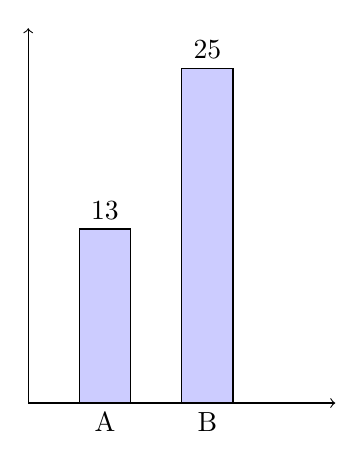
\begin{tikzpicture}[x=0.65cm,y=0.17cm]
\draw[->] (0,0)--(6,0);\draw[->] (0,0)--(0,28.0);
\draw[fill=blue!20] (1,0) rectangle (2,13.0);\node[below] at (1.5,0) {A};\node[above] at (1.5,13.0) {13};
\draw[fill=blue!20] (3,0) rectangle (4,25.0);\node[below] at (3.5,0) {B};\node[above] at (3.5,25.0) {25};
\end{tikzpicture}\end{center}
\textbf{Answer:} \(12\)
\textbf{Method:} Read both bar heights and subtract A from B.
\textbf{Reusable LaTeX template:}
\begin{verbatim}
The bar graph shows books sold on two days. How many more were sold on day B than day A?
\end{verbatim}
\textbf{Answer formula/rule:}
\begin{verbatim}
b-a
\end{verbatim}
\textbf{Generation ranges:} a: 5 to 20; k: 1 to 15
\textbf{Derived variables:} b = a+k
\textbf{Required extensions:} derived\_variables, diagram\_renderer
\medskip\hrule\medskip
\subsection{D10 -- Circle graph sector angle}
\textbf{Targets:} Q.6.a\quad\textbf{Mode:} numeric
\textbf{Question:} A category occupies 75\% of a circle graph. Find its central angle in degrees.
\textbf{Answer:} \(270\)
\textbf{Method:} Multiply the fraction of the whole by 360 degrees.
\textbf{Reusable LaTeX template:}
\begin{verbatim}
A category occupies {p:5–80}\% of a circle graph. Find its central angle in degrees.
\end{verbatim}
\textbf{Answer formula/rule:}
\begin{verbatim}
360*p/100
\end{verbatim}
\textbf{Generation ranges:} p: 5 to 80
\medskip\hrule\medskip
\subsection{D11 -- Histogram frequency}
\textbf{Targets:} Q.6.b\quad\textbf{Mode:} numeric
\textbf{Question:} The histogram shows counts in three score intervals. How many scores lie in the middle interval?
\begin{center}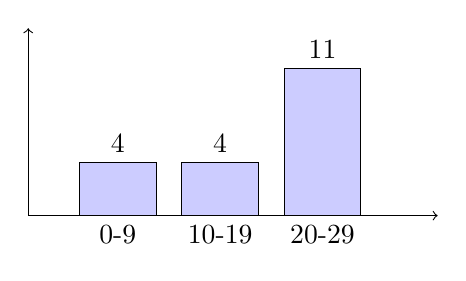
\begin{tikzpicture}[x=0.65cm,y=0.17cm]
\draw[->] (0,0)--(8,0);\draw[->] (0,0)--(0,14.0);
\draw[fill=blue!20] (1,0) rectangle (2.5,4.0);\node[below] at (1.75,0) {0-9};\node[above] at (1.75,4.0) {4};
\draw[fill=blue!20] (3,0) rectangle (4.5,4.0);\node[below] at (3.75,0) {10-19};\node[above] at (3.75,4.0) {4};
\draw[fill=blue!20] (5,0) rectangle (6.5,11.0);\node[below] at (5.75,0) {20-29};\node[above] at (5.75,11.0) {11};
\end{tikzpicture}\end{center}
\textbf{Answer:} \(4\)
\textbf{Method:} Read the height of the middle bin.
\textbf{Reusable LaTeX template:}
\begin{verbatim}
The histogram shows counts in three score intervals. How many scores lie in the middle
interval?
\end{verbatim}
\textbf{Answer formula/rule:}
\begin{verbatim}
b
\end{verbatim}
\textbf{Generation ranges:} a: 2 to 12; b: 2 to 12; c: 2 to 12
\textbf{Required extensions:} diagram\_renderer
\medskip\hrule\medskip
\subsection{D12 -- Box plot interquartile range}
\textbf{Targets:} Q.6.b\quad\textbf{Mode:} numeric
\textbf{Question:} The box plot shows a five-number summary. Find the interquartile range.
\begin{center}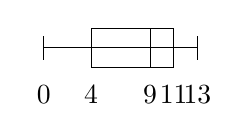
\begin{tikzpicture}[x=0.15cm,y=0.5cm]
\draw (0.0,0)--(13.0,0);\draw (4.0,-0.5) rectangle (11.0,0.5);\draw (9.0,-0.5)--(9.0,0.5);\draw (0.0,-0.3)--(0.0,0.3);\draw (13.0,-0.3)--(13.0,0.3);
\node[below] at (0.0,-0.7) {0};\node[below] at (4.0,-0.7) {4};\node[below] at (9.0,-0.7) {9};\node[below] at (11.0,-0.7) {11};\node[below] at (13.0,-0.7) {13};
\end{tikzpicture}\end{center}
\textbf{Answer:} \(7\)
\textbf{Method:} Subtract Q1 from Q3.
\textbf{Reusable LaTeX template:}
\begin{verbatim}
The box plot shows a five-number summary. Find the interquartile range.
\end{verbatim}
\textbf{Answer formula/rule:}
\begin{verbatim}
q3-q1
\end{verbatim}
\textbf{Generation ranges:} lo: 0 to 10; a: 1 to 8; b: 1 to 8; c: 1 to 8; d: 1 to 8
\textbf{Derived variables:} q1 = lo+a; med = q1+b; q3 = med+c; hi = q3+d
\textbf{Required extensions:} derived\_variables, diagram\_renderer
\medskip\hrule\medskip
\subsection{D13 -- Scatter plot interpretation}
\textbf{Targets:} Q.6.c\quad\textbf{Mode:} category
\textbf{Question:} The plotted points are \((3,3),(4,4),(5,5)\). Classify their association as positive, negative, or neither.
\begin{center}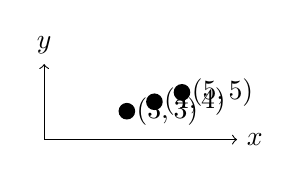
\begin{tikzpicture}[x=0.35cm,y=0.12cm]
\draw[->] (0,0)--(7.0,0) node[right] {$x$};\draw[->] (0,0)--(0,8.0) node[above] {$y$};
\fill (3.0,3.0) circle (3pt);\node[right] at (3.0,3.0) {$(3,3)$};\fill (4.0,4.0) circle (3pt);\node[right] at (4.0,4.0) {$(4,4)$};\fill (5.0,5.0) circle (3pt);\node[right] at (5.0,5.0) {$(5,5)$};
\end{tikzpicture}\end{center}
\textbf{Answer:} \(\text{positive}\)
\textbf{Method:} Both coordinates increase together, so the association is positive.
\textbf{Reusable LaTeX template:}
\begin{verbatim}
The plotted points are \(({a:1–3},{u}),({b},{v}),({c},{w})\). Classify their association
as positive, negative, or neither.
\end{verbatim}
\textbf{Answer formula/rule:}
\begin{verbatim}
positive
\end{verbatim}
\textbf{Generation ranges:} a: 1 to 3; k: 1 to 3; m: 1 to 5; p: 0 to 5
\textbf{Derived variables:} b = a+k; c = b+k; u = m*a+p; v = m*b+p; w = m*c+p
\textbf{Required extensions:} derived\_variables, category\_grading, diagram\_renderer
\medskip\hrule\medskip
\subsection{P01 -- Fundamental counting principle}
\textbf{Targets:} Q.8.a\quad\textbf{Mode:} numeric
\textbf{Question:} A meal offers 5 main dishes, 3 sides, and 5 drinks. Choose one of each. How many meals are possible?
\textbf{Answer:} \(75\)
\textbf{Method:} Multiply the independent numbers of choices.
\textbf{Reusable LaTeX template:}
\begin{verbatim}
A meal offers {a:2–8} main dishes, {b:2–6} sides, and {c:2–5} drinks. Choose one of
each. How many meals are possible?
\end{verbatim}
\textbf{Answer formula/rule:}
\begin{verbatim}
a*b*c
\end{verbatim}
\textbf{Generation ranges:} a: 2 to 8; b: 2 to 6; c: 2 to 5
\medskip\hrule\medskip
\subsection{P02 -- Combinations}
\textbf{Targets:} Q.8.a\quad\textbf{Mode:} numeric
\textbf{Question:} Choose a committee of 5 people from 12 people. Order does not matter. How many committees are possible?
\textbf{Answer:} \(792\)
\textbf{Method:} Use the combination formula n!/(r!(n-r)!).
\textbf{Reusable LaTeX template:}
\begin{verbatim}
Choose a committee of {r:2–5} people from {n:6–15} people. Order does not matter. How
many committees are possible?
\end{verbatim}
\textbf{Answer formula/rule:}
\begin{verbatim}
nCr(n,r)
\end{verbatim}
\textbf{Generation ranges:} n: 6 to 15; r: 2 to 5
\medskip\hrule\medskip
\subsection{P03 -- Permutations}
\textbf{Targets:} Q.8.a\quad\textbf{Mode:} numeric
\textbf{Question:} Assign 5 distinct ranked positions to 9 people, with no person repeated. How many assignments are possible?
\textbf{Answer:} \(15120\)
\textbf{Method:} Use the permutation formula n!/(n-r)!.
\textbf{Reusable LaTeX template:}
\begin{verbatim}
Assign {r:2–5} distinct ranked positions to {n:6–15} people, with no person repeated.
How many assignments are possible?
\end{verbatim}
\textbf{Answer formula/rule:}
\begin{verbatim}
nPr(n,r)
\end{verbatim}
\textbf{Generation ranges:} n: 6 to 15; r: 2 to 5
\medskip\hrule\medskip
\subsection{P04 -- Simple probability}
\textbf{Targets:} Q.8.b\quad\textbf{Mode:} numeric
\textbf{Question:} A bag contains 9 red and 4 blue counters. One is chosen at random. Find the probability of red.
\textbf{Answer:} \(\frac{9}{13}\)
\textbf{Method:} Favorable outcomes divided by total outcomes.
\textbf{Reusable LaTeX template:}
\begin{verbatim}
A bag contains {r:1–12} red and {b:1–12} blue counters. One is chosen at random. Find
the probability of red.
\end{verbatim}
\textbf{Answer formula/rule:}
\begin{verbatim}
r/(r+b)
\end{verbatim}
\textbf{Generation ranges:} r: 1 to 12; b: 1 to 12
\medskip\hrule\medskip
\subsection{P05 -- Independent events with replacement}
\textbf{Targets:} Q.8.b\quad\textbf{Mode:} numeric
\textbf{Question:} A bag contains 6 red and 5 blue counters. Draw twice, replacing the first counter. Find the probability both are red.
\textbf{Answer:} \(\frac{36}{121}\)
\textbf{Method:} The draws are independent; multiply the two probabilities.
\textbf{Reusable LaTeX template:}
\begin{verbatim}
A bag contains {r:1–12} red and {b:1–12} blue counters. Draw twice, replacing the first
counter. Find the probability both are red.
\end{verbatim}
\textbf{Answer formula/rule:}
\begin{verbatim}
pow(r/(r+b),2)
\end{verbatim}
\textbf{Generation ranges:} r: 1 to 12; b: 1 to 12
\medskip\hrule\medskip
\subsection{P06 -- Dependent events without replacement}
\textbf{Targets:} Q.8.b\quad\textbf{Mode:} numeric
\textbf{Question:} A bag contains 12 red and 3 blue counters. Draw twice without replacement. Find the probability both are red.
\textbf{Answer:} \(\frac{22}{35}\)
\textbf{Method:} After the first red draw, one fewer red and total counter remain.
\textbf{Reusable LaTeX template:}
\begin{verbatim}
A bag contains {r:2–12} red and {b:1–12} blue counters. Draw twice without replacement.
Find the probability both are red.
\end{verbatim}
\textbf{Answer formula/rule:}
\begin{verbatim}
r/(r+b)*(r-1)/(r+b-1)
\end{verbatim}
\textbf{Generation ranges:} r: 2 to 12; b: 1 to 12
\medskip\hrule\medskip
\subsection{P07 -- Complement probability}
\textbf{Targets:} Q.8.b\quad\textbf{Mode:} numeric
\textbf{Question:} The probability of rain is \(\frac{1}{8}\). Find the probability of no rain.
\textbf{Answer:} \(0.875\)
\textbf{Method:} Subtract the event probability from one.
\textbf{Reusable LaTeX template:}
\begin{verbatim}
The probability of rain is \(\frac{{a:1–5}}{{b:6–12}}\). Find the probability of no
rain.
\end{verbatim}
\textbf{Answer formula/rule:}
\begin{verbatim}
1-a/b
\end{verbatim}
\textbf{Generation ranges:} a: 1 to 5; b: 6 to 12
\medskip\hrule\medskip
\section{Expressions and polynomials}
\subsection{E01 -- Combine like terms}
\textbf{Targets:} A.1.a\quad\textbf{Mode:} expression
\textbf{Question:} Simplify \(4x+6x+6\).
\textbf{Answer:} \(10x+(6)\)
\textbf{Method:} Add the coefficients of x.
\textbf{Reusable LaTeX template:}
\begin{verbatim}
Simplify \({a:1–10}x+{b:1–10}x+{c:-10–10}\).
\end{verbatim}
\textbf{Answer formula/rule:}
\begin{verbatim}
(a+b)*x+c
\end{verbatim}
\textbf{Generation ranges:} a: 1 to 10; b: 1 to 10; c: -10 to 10
\textbf{Derived variables:} coef = a+b
\textbf{Required extensions:} expression\_grading, derived\_variables
\medskip\hrule\medskip
\subsection{E02 -- Distribute a coefficient}
\textbf{Targets:} A.1.a\quad\textbf{Mode:} expression
\textbf{Question:} Expand \(10(10x+2)\).
\textbf{Answer:} \(100x+20\)
\textbf{Method:} Multiply both terms by the outside coefficient.
\textbf{Reusable LaTeX template:}
\begin{verbatim}
Expand \({a:2–10}({b:1–10}x+{c:1–10})\).
\end{verbatim}
\textbf{Answer formula/rule:}
\begin{verbatim}
a*b*x+a*c
\end{verbatim}
\textbf{Generation ranges:} a: 2 to 10; b: 1 to 10; c: 1 to 10
\textbf{Derived variables:} coef = a*b; constant = a*c
\textbf{Required extensions:} expression\_grading, derived\_variables
\medskip\hrule\medskip
\subsection{E03 -- Evaluate a linear expression}
\textbf{Targets:} A.1.b\quad\textbf{Mode:} numeric
\textbf{Question:} Evaluate \(-6x+9\) at \(x=4\).
\textbf{Answer:} \(-15\)
\textbf{Method:} Substitute v for x and calculate.
\textbf{Reusable LaTeX template:}
\begin{verbatim}
Evaluate \({a:-10–10}x+{b:-20–20}\) at \(x={v:-10–10}\).
\end{verbatim}
\textbf{Answer formula/rule:}
\begin{verbatim}
a*v+b
\end{verbatim}
\textbf{Generation ranges:} a: -10 to 10; b: -20 to 20; v: -10 to 10
\medskip\hrule\medskip
\subsection{E04 -- Translate a linear cost expression}
\textbf{Targets:} A.1.c\quad\textbf{Mode:} expression
\textbf{Question:} A rental has a fixed fee of \(\$18\) plus \(\$5\) per hour. Write total cost as an expression in hours \(h\).
\textbf{Answer:} \(5h+18\)
\textbf{Method:} Variable cost plus fixed fee.
\textbf{Reusable LaTeX template:}
\begin{verbatim}
A rental has a fixed fee of \(\${b:5–50}\) plus \(\${a:2–20}\) per hour. Write total
cost as an expression in hours \(h\).
\end{verbatim}
\textbf{Answer formula/rule:}
\begin{verbatim}
a*h+b
\end{verbatim}
\textbf{Generation ranges:} a: 2 to 20; b: 5 to 50
\textbf{Required extensions:} expression\_grading
\medskip\hrule\medskip
\subsection{E05 -- Add polynomials}
\textbf{Targets:} A.1.d\quad\textbf{Mode:} expression
\textbf{Question:} Simplify \((2x^2+1x+5)+(6x^2+3x+5)\).
\textbf{Answer:} \(8x^2+4x+10\)
\textbf{Method:} Combine terms with the same power of x.
\textbf{Reusable LaTeX template:}
\begin{verbatim}
Simplify \(({a:1–8}x^2+{b:1–8}x+{c:1–8})+({d:1–8}x^2+{e:1–8}x+{f:1–8})\).
\end{verbatim}
\textbf{Answer formula/rule:}
\begin{verbatim}
(a+d)*x*x+(b+e)*x+c+f
\end{verbatim}
\textbf{Generation ranges:} a: 1 to 8; b: 1 to 8; c: 1 to 8; d: 1 to 8; e: 1 to 8; f: 1 to 8
\textbf{Derived variables:} coef2 = a+d; coef1 = b+e; constant = c+f
\textbf{Required extensions:} expression\_grading, derived\_variables
\medskip\hrule\medskip
\subsection{E06 -- Subtract polynomials}
\textbf{Targets:} A.1.d\quad\textbf{Mode:} expression
\textbf{Question:} Simplify \((1x^2+6x+4)-(1x^2+6x+3)\).
\textbf{Answer:} \((0)x^2+(0)x+(1)\)
\textbf{Method:} Distribute the minus sign before combining terms.
\textbf{Reusable LaTeX template:}
\begin{verbatim}
Simplify \(({a:1–8}x^2+{b:1–8}x+{c:1–8})-({d:1–8}x^2+{e:1–8}x+{f:1–8})\).
\end{verbatim}
\textbf{Answer formula/rule:}
\begin{verbatim}
(a-d)*x*x+(b-e)*x+c-f
\end{verbatim}
\textbf{Generation ranges:} a: 1 to 8; b: 1 to 8; c: 1 to 8; d: 1 to 8; e: 1 to 8; f: 1 to 8
\textbf{Derived variables:} coef2 = a-d; coef1 = b-e; constant = c-f
\textbf{Required extensions:} expression\_grading, derived\_variables
\medskip\hrule\medskip
\subsection{E07 -- Multiply binomials}
\textbf{Targets:} A.1.d\quad\textbf{Mode:} expression
\textbf{Question:} Expand \((x+9)(x+6)\).
\textbf{Answer:} \(x^2+15x+54\)
\textbf{Method:} Multiply all pairs of terms and combine.
\textbf{Reusable LaTeX template:}
\begin{verbatim}
Expand \((x+{a:1–12})(x+{b:1–12})\).
\end{verbatim}
\textbf{Answer formula/rule:}
\begin{verbatim}
x*x+(a+b)*x+a*b
\end{verbatim}
\textbf{Generation ranges:} a: 1 to 12; b: 1 to 12
\textbf{Derived variables:} coef = a+b; constant = a*b
\textbf{Required extensions:} expression\_grading, derived\_variables
\medskip\hrule\medskip
\subsection{E08 -- Divide factorable polynomials}
\textbf{Targets:} A.1.d\quad\textbf{Mode:} expression
\textbf{Question:} Simplify \(\frac{x^2-49}{x-7}\), retaining the restriction \(x\ne 7\).
\textbf{Answer:} \(x+7,\quad x\ne 7\)
\textbf{Method:} Factor the numerator as (x-a)(x+a); preserve the original domain.
\textbf{Reusable LaTeX template:}
\begin{verbatim}
Simplify \(\frac{x^2-{k}}{x-{a:1–12}}\), retaining the restriction \(x\ne {a}\).
\end{verbatim}
\textbf{Answer formula/rule:}
\begin{verbatim}
x+a
\end{verbatim}
\textbf{Generation ranges:} a: 1 to 12
\textbf{Derived variables:} k = a*a
\textbf{Required extensions:} derived\_variables, expression\_grading
\medskip\hrule\medskip
\subsection{E09 -- Evaluate a polynomial}
\textbf{Targets:} A.1.e\quad\textbf{Mode:} numeric
\textbf{Question:} Evaluate \(6x^2+-5x+-19\) at \(x=-1\).
\textbf{Answer:} \(-8\)
\textbf{Method:} Substitute v for x, square before multiplying.
\textbf{Reusable LaTeX template:}
\begin{verbatim}
Evaluate \({a:1–8}x^2+{b:-10–10}x+{c:-20–20}\) at \(x={v:-6–6}\).
\end{verbatim}
\textbf{Answer formula/rule:}
\begin{verbatim}
a*v*v+b*v+c
\end{verbatim}
\textbf{Generation ranges:} a: 1 to 8; b: -10 to 10; c: -20 to 20; v: -6 to 6
\medskip\hrule\medskip
\subsection{E10 -- Factor a common factor}
\textbf{Targets:} A.1.f\quad\textbf{Mode:} factored\_expression
\textbf{Question:} Factor completely over the integers: \(24x+15\).
\textbf{Answer:} \(3(8x+5)\)
\textbf{Method:} Take out the greatest common factor; the remaining coefficients are coprime.
\textbf{Reusable LaTeX template:}
\begin{verbatim}
Factor completely over the integers: \({A}x+{B}\).
\end{verbatim}
\textbf{Answer formula/rule:}
\begin{verbatim}
g*(a*x+b)
\end{verbatim}
\textbf{Generation ranges:} g: 2 to 10; a: 1 to 9; b: 1 to 9
\textbf{Derived variables:} A = g*a; B = g*b
\textbf{Constraints:} gcd(a,b)==1
\textbf{Required extensions:} derived\_variables, constraint\_filtering, factored\_expression\_grading
\medskip\hrule\medskip
\subsection{E11 -- Factor a monic quadratic}
\textbf{Targets:} A.1.f\quad\textbf{Mode:} factored\_expression
\textbf{Question:} Factor completely: \(x^2+18x+72\).
\textbf{Answer:} \((x+6)(x+12)\)
\textbf{Method:} Find two integers whose sum is s and product is p.
\textbf{Reusable LaTeX template:}
\begin{verbatim}
Factor completely: \(x^2+{s}x+{p}\).
\end{verbatim}
\textbf{Answer formula/rule:}
\begin{verbatim}
(x+a)*(x+b)
\end{verbatim}
\textbf{Generation ranges:} a: 1 to 12; b: 1 to 12
\textbf{Derived variables:} s = a+b; p = a*b
\textbf{Required extensions:} derived\_variables, factored\_expression\_grading
\medskip\hrule\medskip
\subsection{E12 -- Factor difference of squares}
\textbf{Targets:} A.1.f\quad\textbf{Mode:} factored\_expression
\textbf{Question:} Factor completely: \(x^2-36\).
\textbf{Answer:} \((x-6)(x+6)\)
\textbf{Method:} Use the difference-of-squares identity.
\textbf{Reusable LaTeX template:}
\begin{verbatim}
Factor completely: \(x^2-{k}\).
\end{verbatim}
\textbf{Answer formula/rule:}
\begin{verbatim}
(x-a)*(x+a)
\end{verbatim}
\textbf{Generation ranges:} a: 1 to 12
\textbf{Derived variables:} k = a*a
\textbf{Required extensions:} derived\_variables, factored\_expression\_grading
\medskip\hrule\medskip
\subsection{E13 -- Translate a polynomial area expression}
\textbf{Targets:} A.1.g\quad\textbf{Mode:} expression
\textbf{Question:} A rectangle has side lengths \(x+4\) and \(x+4\), where \(x\ge0\). Write its area as a polynomial in \(x\).
\textbf{Answer:} \(x^2+8x+16\)
\textbf{Method:} Multiply length and width, then expand.
\textbf{Reusable LaTeX template:}
\begin{verbatim}
A rectangle has side lengths \(x+{a:1–12}\) and \(x+{b:1–12}\), where \(x\ge0\). Write
its area as a polynomial in \(x\).
\end{verbatim}
\textbf{Answer formula/rule:}
\begin{verbatim}
x*x+(a+b)*x+a*b
\end{verbatim}
\textbf{Generation ranges:} a: 1 to 12; b: 1 to 12
\textbf{Derived variables:} coef = a+b; constant = a*b
\textbf{Required extensions:} expression\_grading, derived\_variables
\medskip\hrule\medskip
\subsection{E14 -- Add rational expressions}
\textbf{Targets:} A.1.h\quad\textbf{Mode:} expression
\textbf{Question:} Simplify \(\frac{11}{x}+\frac{8}{x}\), where \(x\ne0\).
\textbf{Answer:} \(\frac{19}{x},\quad x\ne0\)
\textbf{Method:} Add numerators over the common denominator.
\textbf{Reusable LaTeX template:}
\begin{verbatim}
Simplify \(\frac{{a:1–12}}{x}+\frac{{b:1–12}}{x}\), where \(x\ne0\).
\end{verbatim}
\textbf{Answer formula/rule:}
\begin{verbatim}
(a+b)/x
\end{verbatim}
\textbf{Generation ranges:} a: 1 to 12; b: 1 to 12
\textbf{Derived variables:} total = a+b
\textbf{Required extensions:} expression\_grading, derived\_variables
\medskip\hrule\medskip
\subsection{E15 -- Multiply rational expressions}
\textbf{Targets:} A.1.h\quad\textbf{Mode:} numeric
\textbf{Question:} Simplify \(\frac{6x}{6}\cdot\frac{12}{1x}\), where \(x\ne0\).
\textbf{Answer:} \(12\)
\textbf{Method:} Cancel nonzero x, multiply numerators and denominators.
\textbf{Reusable LaTeX template:}
\begin{verbatim}
Simplify \(\frac{{a:1–12}x}{{b:1–12}}\cdot\frac{{c:1–12}}{{d:1–12}x}\), where \(x\ne0\).
\end{verbatim}
\textbf{Answer formula/rule:}
\begin{verbatim}
a*c/(b*d)
\end{verbatim}
\textbf{Generation ranges:} a: 1 to 12; b: 1 to 12; c: 1 to 12; d: 1 to 12
\medskip\hrule\medskip
\subsection{E16 -- Evaluate a rational expression}
\textbf{Targets:} A.1.i\quad\textbf{Mode:} numeric
\textbf{Question:} Evaluate \(\frac{2x+8}{x+5}\) at \(x=1\).
\textbf{Answer:} \(\frac{5}{3}\)
\textbf{Method:} Substitute v; the generated denominator is positive.
\textbf{Reusable LaTeX template:}
\begin{verbatim}
Evaluate \(\frac{{a:1–10}x+{b:1–15}}{x+{c:1–10}}\) at \(x={v:0–10}\).
\end{verbatim}
\textbf{Answer formula/rule:}
\begin{verbatim}
(a*v+b)/(v+c)
\end{verbatim}
\textbf{Generation ranges:} a: 1 to 10; b: 1 to 15; c: 1 to 10; v: 0 to 10
\medskip\hrule\medskip
\subsection{E17 -- Translate a rational rate expression}
\textbf{Targets:} A.1.j\quad\textbf{Mode:} expression
\textbf{Question:} A trip covers 238 miles in \(t\) hours, with \(t>0\). Write the average speed as an expression in \(t\).
\textbf{Answer:} \(\frac{238}{t},\quad t>0\)
\textbf{Method:} Average speed equals distance divided by time.
\textbf{Reusable LaTeX template:}
\begin{verbatim}
A trip covers {d:20–300} miles in \(t\) hours, with \(t>0\). Write the average speed as
an expression in \(t\).
\end{verbatim}
\textbf{Answer formula/rule:}
\begin{verbatim}
d/t
\end{verbatim}
\textbf{Generation ranges:} d: 20 to 300
\textbf{Required extensions:} expression\_grading
\medskip\hrule\medskip
\section{Linear equations and systems}
\subsection{L01 -- One-step addition equation}
\textbf{Targets:} A.2.a\quad\textbf{Mode:} numeric
\textbf{Question:} Solve \(x+1=10\).
\textbf{Answer:} \(9\)
\textbf{Method:} Subtract b from both sides.
\textbf{Reusable LaTeX template:}
\begin{verbatim}
Solve \(x+{b:-20–20}={c:-20–20}\).
\end{verbatim}
\textbf{Answer formula/rule:}
\begin{verbatim}
c-b
\end{verbatim}
\textbf{Generation ranges:} b: -20 to 20; c: -20 to 20
\medskip\hrule\medskip
\subsection{L02 -- One-step multiplication equation}
\textbf{Targets:} A.2.a\quad\textbf{Mode:} numeric
\textbf{Question:} Solve \(5x=19\).
\textbf{Answer:} \(3.8\)
\textbf{Method:} Divide both sides by a.
\textbf{Reusable LaTeX template:}
\begin{verbatim}
Solve \({a:1–12}x={b:-30–30}\).
\end{verbatim}
\textbf{Answer formula/rule:}
\begin{verbatim}
b/a
\end{verbatim}
\textbf{Generation ranges:} a: 1 to 12; b: -30 to 30
\medskip\hrule\medskip
\subsection{L03 -- Two-step equation}
\textbf{Targets:} A.2.a\quad\textbf{Mode:} numeric
\textbf{Question:} Solve \(11x+(-13)=-15\).
\textbf{Answer:} \(\frac{-2}{11}\)
\textbf{Method:} Subtract b and divide by a.
\textbf{Reusable LaTeX template:}
\begin{verbatim}
Solve \({a:1–12}x+({b:-20–20})={c:-30–30}\).
\end{verbatim}
\textbf{Answer formula/rule:}
\begin{verbatim}
(c-b)/a
\end{verbatim}
\textbf{Generation ranges:} a: 1 to 12; b: -20 to 20; c: -30 to 30
\medskip\hrule\medskip
\subsection{L04 -- Equation with parentheses}
\textbf{Targets:} A.2.a\quad\textbf{Mode:} numeric
\textbf{Question:} Solve \(4(x+10)=93\).
\textbf{Answer:} \(13.25\)
\textbf{Method:} Divide by a, then subtract b.
\textbf{Reusable LaTeX template:}
\begin{verbatim}
Solve \({a:2–10}(x+{b:1–12})={c:1–100}\).
\end{verbatim}
\textbf{Answer formula/rule:}
\begin{verbatim}
c/a-b
\end{verbatim}
\textbf{Generation ranges:} a: 2 to 10; b: 1 to 12; c: 1 to 100
\medskip\hrule\medskip
\subsection{L05 -- Variables on both sides}
\textbf{Targets:} A.2.a\quad\textbf{Mode:} numeric
\textbf{Question:} Solve \(12x+-1=8x+11\).
\textbf{Answer:} \(3\)
\textbf{Method:} Collect x terms; a-c is nonzero by construction.
\textbf{Reusable LaTeX template:}
\begin{verbatim}
Solve \({a}x+{b:-20–20}={c:1–8}x+{d:-20–20}\).
\end{verbatim}
\textbf{Answer formula/rule:}
\begin{verbatim}
(d-b)/(a-c)
\end{verbatim}
\textbf{Generation ranges:} c: 1 to 8; k: 1 to 8; b: -20 to 20; d: -20 to 20
\textbf{Derived variables:} a = c+k
\textbf{Required extensions:} derived\_variables
\medskip\hrule\medskip
\subsection{L06 -- Rational-coefficient equation}
\textbf{Targets:} A.2.a\quad\textbf{Mode:} numeric
\textbf{Question:} Solve \(\frac{10}{5}x+-8=-9\).
\textbf{Answer:} \(-0.5\)
\textbf{Method:} Subtract c, then multiply by b/a.
\textbf{Reusable LaTeX template:}
\begin{verbatim}
Solve \(\frac{{a:1–10}}{{b:2–12}}x+{c:-10–10}={d:-20–20}\).
\end{verbatim}
\textbf{Answer formula/rule:}
\begin{verbatim}
(d-c)*b/a
\end{verbatim}
\textbf{Generation ranges:} a: 1 to 10; b: 2 to 12; c: -10 to 10; d: -20 to 20
\medskip\hrule\medskip
\subsection{L07 -- Literal equation}
\textbf{Targets:} A.2.a\quad\textbf{Mode:} expression
\textbf{Question:} Rearrange \(y=ax+b\) to solve for \(x\), assuming \(a\ne0\).
\textbf{Answer:} \(x=\frac{y-b}{a}\)
\textbf{Method:} Subtract b and divide by a; this template has symbolic coefficients.
\textbf{Reusable LaTeX template:}
\begin{verbatim}
Rearrange \(y=ax+b\) to solve for \(x\), assuming \(a\ne0\).
\end{verbatim}
\textbf{Answer formula/rule:}
\begin{verbatim}
(y-b)/a
\end{verbatim}
\textbf{Generation ranges:} Symbolic coefficients; no sampled variables.
\textbf{Required extensions:} expression\_grading
\medskip\hrule\medskip
\subsection{L08 -- Rental time from total cost}
\textbf{Targets:} A.2.b\quad\textbf{Mode:} numeric
\textbf{Question:} A rental costs \(\$24\) plus \(\$12\) per hour. The total is \(\$144\). Find the rental time in hours.
\textbf{Answer:} \(10\)
\textbf{Method:} Set variable cost plus fixed fee equal to the total.
\textbf{Reusable LaTeX template:}
\begin{verbatim}
A rental costs \(\${b:5–50}\) plus \(\${a:2–20}\) per hour. The total is \(\${c}\). Find
the rental time in hours.
\end{verbatim}
\textbf{Answer formula/rule:}
\begin{verbatim}
(c-b)/a
\end{verbatim}
\textbf{Generation ranges:} a: 2 to 20; b: 5 to 50; h: 1 to 12
\textbf{Derived variables:} c = a*h+b
\textbf{Required extensions:} derived\_variables
\medskip\hrule\medskip
\subsection{L09 -- Write a cost equation}
\textbf{Targets:} A.2.c\quad\textbf{Mode:} equation
\textbf{Question:} A service charges \(\$26\) plus \(\$6\) per hour. Write an equation for total cost \(C\) in hours \(h\).
\textbf{Answer:} \(C=6h+26\)
\textbf{Method:} Relate total cost to hours and the fixed charge.
\textbf{Reusable LaTeX template:}
\begin{verbatim}
A service charges \(\${b:5–50}\) plus \(\${a:2–20}\) per hour. Write an equation for
total cost \(C\) in hours \(h\).
\end{verbatim}
\textbf{Answer formula/rule:}
\begin{verbatim}
C=a*h+b
\end{verbatim}
\textbf{Generation ranges:} a: 2 to 20; b: 5 to 50
\textbf{Required extensions:} equation\_grading
\medskip\hrule\medskip
\subsection{L10 -- Write a two-variable purchase equation}
\textbf{Targets:} A.2.c\quad\textbf{Mode:} equation
\textbf{Question:} Adult tickets cost \(\$11\), child tickets cost \(\$4\), and total revenue is \(\$41\). Write an equation using adult count \(x\) and child count \(y\).
\textbf{Answer:} \(11x+4y=41\)
\textbf{Method:} Sum the revenue from the two ticket types.
\textbf{Reusable LaTeX template:}
\begin{verbatim}
Adult tickets cost \(\${a:10–20}\), child tickets cost \(\${b:3–9}\), and total revenue
is \(\${t}\). Write an equation using adult count \(x\) and child count \(y\).
\end{verbatim}
\textbf{Answer formula/rule:}
\begin{verbatim}
a*x+b*y=t
\end{verbatim}
\textbf{Generation ranges:} a: 10 to 20; b: 3 to 9; u: 2 to 10; v: 2 to 10
\textbf{Derived variables:} t = a*u+b*v
\textbf{Required extensions:} derived\_variables, equation\_grading
\medskip\hrule\medskip
\subsection{L11 -- Solve a system: x component}
\textbf{Targets:} A.2.d\quad\textbf{Mode:} numeric
\textbf{Question:} Solve \(x+y=5\), \(7x+2y=20\). Enter only \(x\).
\textbf{Answer:} \(2\)
\textbf{Method:} Substitute y=s-x in the second equation.
\textbf{Reusable LaTeX template:}
\begin{verbatim}
Solve \(x+y={s}\), \({a}x+{b:1–5}y={t}\). Enter only \(x\).
\end{verbatim}
\textbf{Answer formula/rule:}
\begin{verbatim}
(t-b*s)/(a-b)
\end{verbatim}
\textbf{Generation ranges:} b: 1 to 5; k: 1 to 5; u: 1 to 10; v: 1 to 10
\textbf{Derived variables:} a = b+k; s = u+v; t = a*u+b*v
\textbf{Required extensions:} derived\_variables
\medskip\hrule\medskip
\subsection{L12 -- Solve a system: ordered pair}
\textbf{Targets:} A.2.d\quad\textbf{Mode:} ordered\_pair
\textbf{Question:} Solve \(x+y=17\), \(6x+2y=70\). Enter \((x,y)\).
\textbf{Answer:} \((9,8)\)
\textbf{Method:} Eliminate one variable, then substitute to find the other.
\textbf{Reusable LaTeX template:}
\begin{verbatim}
Solve \(x+y={s}\), \({a}x+{b:1–5}y={t}\). Enter \((x,y)\).
\end{verbatim}
\textbf{Answer formula/rule:}
\begin{verbatim}
[u,v]
\end{verbatim}
\textbf{Generation ranges:} b: 1 to 5; k: 1 to 5; u: 1 to 10; v: 1 to 10
\textbf{Derived variables:} a = b+k; s = u+v; t = a*u+b*v
\textbf{Required extensions:} derived\_variables, ordered\_pair\_grading
\medskip\hrule\medskip
\subsection{L13 -- Ticket system word problem}
\textbf{Targets:} A.2.d\quad\textbf{Mode:} numeric
\textbf{Question:} 9 tickets were sold. Adult tickets cost \(\$6\), child tickets cost \(\$4\), and revenue was \(\$42\). How many adult tickets were sold?
\textbf{Answer:} \(3\)
\textbf{Method:} Use the ticket-count and revenue equations.
\textbf{Reusable LaTeX template:}
\begin{verbatim}
{s} tickets were sold. Adult tickets cost \(\${a}\), child tickets cost \(\${b:3–8}\),
and revenue was \(\${t}\). How many adult tickets were sold?
\end{verbatim}
\textbf{Answer formula/rule:}
\begin{verbatim}
(t-b*s)/(a-b)
\end{verbatim}
\textbf{Generation ranges:} b: 3 to 8; k: 2 to 8; u: 2 to 20; v: 2 to 20
\textbf{Derived variables:} a = b+k; s = u+v; t = a*u+b*v
\textbf{Required extensions:} derived\_variables
\medskip\hrule\medskip
\section{Linear inequalities}
\subsection{I01 -- Solve a positive-coefficient inequality}
\textbf{Targets:} A.3.a\quad\textbf{Mode:} inequality
\textbf{Question:} Solve \(3x+3<-1\).
\textbf{Answer:} \(x<\frac{-1-(3)}{3}\)
\textbf{Method:} Subtract b and divide by positive a; keep the inequality direction.
\textbf{Reusable LaTeX template:}
\begin{verbatim}
Solve \({a:1–10}x+{b:-20–20}<{c:-20–20}\).
\end{verbatim}
\textbf{Answer formula/rule:}
\begin{verbatim}
x < (c-b)/a
\end{verbatim}
\textbf{Generation ranges:} a: 1 to 10; b: -20 to 20; c: -20 to 20
\textbf{Required extensions:} inequality\_grading
\medskip\hrule\medskip
\subsection{I02 -- Solve a negative-coefficient inequality}
\textbf{Targets:} A.3.a\quad\textbf{Mode:} inequality
\textbf{Question:} Solve \(-5x+13\le -2\).
\textbf{Answer:} \(x\ge\frac{13-(-2)}{5}\)
\textbf{Method:} Dividing by a negative coefficient reverses the inequality.
\textbf{Reusable LaTeX template:}
\begin{verbatim}
Solve \(-{a:1–10}x+{b:-20–20}\le {c:-20–20}\).
\end{verbatim}
\textbf{Answer formula/rule:}
\begin{verbatim}
x >= (b-c)/a
\end{verbatim}
\textbf{Generation ranges:} a: 1 to 10; b: -20 to 20; c: -20 to 20
\textbf{Required extensions:} inequality\_grading
\medskip\hrule\medskip
\subsection{I03 -- Graph a strict inequality}
\textbf{Targets:} A.3.b\quad\textbf{Mode:} number\_line
\textbf{Question:} Graph \(x>-10\) on a number line.
\textbf{Answer:} \((-10,\infty)\)
\textbf{Method:} Use an open circle at a and shade to the right.
\textbf{Reusable LaTeX template:}
\begin{verbatim}
Graph \(x>{a:-10–10}\) on a number line.
\end{verbatim}
\textbf{Answer formula/rule:}
\begin{verbatim}
open endpoint a; shade right
\end{verbatim}
\textbf{Generation ranges:} a: -10 to 10
\textbf{Required extensions:} number\_line\_grading
\medskip\hrule\medskip
\subsection{I04 -- Graph an inclusive inequality}
\textbf{Targets:} A.3.b\quad\textbf{Mode:} number\_line
\textbf{Question:} Graph \(x\le 5\) on a number line.
\textbf{Answer:} \((-\infty,5]\)
\textbf{Method:} Use a filled circle at a and shade to the left.
\textbf{Reusable LaTeX template:}
\begin{verbatim}
Graph \(x\le {a:-10–10}\) on a number line.
\end{verbatim}
\textbf{Answer formula/rule:}
\begin{verbatim}
closed endpoint a; shade left
\end{verbatim}
\textbf{Generation ranges:} a: -10 to 10
\textbf{Required extensions:} number\_line\_grading
\medskip\hrule\medskip
\subsection{I05 -- Budget maximum whole items}
\textbf{Targets:} A.3.c\quad\textbf{Mode:} numeric
\textbf{Question:} You have \(\$181\), pay a fixed fee of \(\$20\), and each item costs \(\$14\). What is the maximum whole number of items you can buy?
\textbf{Answer:} \(11\)
\textbf{Method:} Solve f+p*n <= B, then take the floor.
\textbf{Reusable LaTeX template:}
\begin{verbatim}
You have \(\${B:50–200}\), pay a fixed fee of \(\${f:5–20}\), and each item costs
\(\${p:2–15}\). What is the maximum whole number of items you can buy?
\end{verbatim}
\textbf{Answer formula/rule:}
\begin{verbatim}
floor((B-f)/p)
\end{verbatim}
\textbf{Generation ranges:} B: 50 to 200; f: 5 to 20; p: 2 to 15
\medskip\hrule\medskip
\subsection{I06 -- Write a budget inequality}
\textbf{Targets:} A.3.d\quad\textbf{Mode:} inequality
\textbf{Question:} A fixed fee is \(\$16\), each item costs \(\$7\), and the budget is \(\$130\). Write an inequality for the nonnegative whole number \(n\) of items.
\textbf{Answer:} \(16+7n\le 130,\quad n\in\mathbb Z_{\ge0}\)
\textbf{Method:} Total cost must not exceed the budget; counts are nonnegative integers.
\textbf{Reusable LaTeX template:}
\begin{verbatim}
A fixed fee is \(\${f:5–20}\), each item costs \(\${p:2–15}\), and the budget is
\(\${B:50–200}\). Write an inequality for the nonnegative whole number \(n\) of items.
\end{verbatim}
\textbf{Answer formula/rule:}
\begin{verbatim}
f+p*n <= B
\end{verbatim}
\textbf{Generation ranges:} B: 50 to 200; f: 5 to 20; p: 2 to 15
\textbf{Required extensions:} inequality\_grading
\medskip\hrule\medskip
\section{Quadratic equations}
\subsection{Q01 -- Quadratic square equation, positive root}
\textbf{Targets:} A.4.a\quad\textbf{Mode:} numeric
\textbf{Question:} Solve \(x^2=196\). Enter only the positive solution.
\textbf{Answer:} \(14\)
\textbf{Method:} The solutions are plus/minus a; only the positive one is requested.
\textbf{Reusable LaTeX template:}
\begin{verbatim}
Solve \(x^2={k}\). Enter only the positive solution.
\end{verbatim}
\textbf{Answer formula/rule:}
\begin{verbatim}
a
\end{verbatim}
\textbf{Generation ranges:} a: 1 to 20
\textbf{Derived variables:} k = a*a
\textbf{Required extensions:} derived\_variables
\medskip\hrule\medskip
\subsection{Q02 -- Factorable quadratic, all real roots}
\textbf{Targets:} A.4.a\quad\textbf{Mode:} solution\_set
\textbf{Question:} Solve \(x^2-(11)x+(10)=0\). Enter all distinct real solutions.
\textbf{Answer:} \(\left\{1, 10\right\}\)
\textbf{Method:} Factor as (x-a)(x-b); repeated roots count once.
\textbf{Reusable LaTeX template:}
\begin{verbatim}
Solve \(x^2-({s})x+({p})=0\). Enter all distinct real solutions.
\end{verbatim}
\textbf{Answer formula/rule:}
\begin{verbatim}
set([a,b])
\end{verbatim}
\textbf{Generation ranges:} a: -12 to 12; b: -12 to 12
\textbf{Derived variables:} s = a+b; p = a*b
\textbf{Required extensions:} derived\_variables, solution\_set\_grading
\medskip\hrule\medskip
\subsection{Q03 -- Quadratic formula, larger root}
\textbf{Targets:} A.4.a\quad\textbf{Mode:} numeric
\textbf{Question:} Solve \(x^2-(8)x+(-48)=0\). Enter only the larger real solution.
\textbf{Answer:} \(12\)
\textbf{Method:} Use the plus sign in the quadratic formula for a monic quadratic.
\textbf{Reusable LaTeX template:}
\begin{verbatim}
Solve \(x^2-({s})x+({p})=0\). Enter only the larger real solution.
\end{verbatim}
\textbf{Answer formula/rule:}
\begin{verbatim}
(s+sqrt(s*s-4*p))/2
\end{verbatim}
\textbf{Generation ranges:} a: -12 to 12; b: -12 to 12
\textbf{Derived variables:} s = a+b; p = a*b
\textbf{Required extensions:} derived\_variables
\medskip\hrule\medskip
\subsection{Q04 -- Complete the square}
\textbf{Targets:} A.4.a\quad\textbf{Mode:} solution\_set
\textbf{Question:} Solve \((x-(-9))^2=16\). Enter both real solutions.
\textbf{Answer:} \(\left\{-13, -5\right\}\)
\textbf{Method:} Take both square-root signs before adding h.
\textbf{Reusable LaTeX template:}
\begin{verbatim}
Solve \((x-({h:-10–10}))^2={k}\). Enter both real solutions.
\end{verbatim}
\textbf{Answer formula/rule:}
\begin{verbatim}
set([h-a,h+a])
\end{verbatim}
\textbf{Generation ranges:} h: -10 to 10; a: 1 to 10
\textbf{Derived variables:} k = a*a
\textbf{Required extensions:} derived\_variables, solution\_set\_grading
\medskip\hrule\medskip
\subsection{Q05 -- Repeated quadratic root}
\textbf{Targets:} A.4.a\quad\textbf{Mode:} numeric
\textbf{Question:} Solve \(x^2-(-2)x+(1)=0\).
\textbf{Answer:} \(-1\)
\textbf{Method:} The quadratic is (x-a) squared, so there is one distinct root.
\textbf{Reusable LaTeX template:}
\begin{verbatim}
Solve \(x^2-({s})x+({p})=0\).
\end{verbatim}
\textbf{Answer formula/rule:}
\begin{verbatim}
a
\end{verbatim}
\textbf{Generation ranges:} a: -12 to 12
\textbf{Derived variables:} s = 2*a; p = a*a
\textbf{Required extensions:} derived\_variables
\medskip\hrule\medskip
\subsection{Q06 -- Write a quadratic area equation}
\textbf{Targets:} A.4.b\quad\textbf{Mode:} equation
\textbf{Question:} A rectangle has sides \(x\) and \(x+9\) cm and area 190 square centimeters. Write a quadratic equation for \(x>0\).
\textbf{Answer:} \(x^2+9x=190,\quad x>0\)
\textbf{Method:} Multiply the two side lengths and equate to the area.
\textbf{Reusable LaTeX template:}
\begin{verbatim}
A rectangle has sides \(x\) and \(x+{d:1–10}\) cm and area {A} square centimeters. Write
a quadratic equation for \(x>0\).
\end{verbatim}
\textbf{Answer formula/rule:}
\begin{verbatim}
x*x+d*x=A
\end{verbatim}
\textbf{Generation ranges:} d: 1 to 10; u: 2 to 15
\textbf{Derived variables:} A = u*(u+d)
\textbf{Required extensions:} derived\_variables, equation\_grading
\medskip\hrule\medskip
\subsection{Q07 -- Quadratic area word problem}
\textbf{Targets:} A.4.a, A.4.b\quad\textbf{Mode:} numeric
\textbf{Question:} A rectangle has sides \(x\) and \(x+10\) cm and area 299 square centimeters. Find the positive value of \(x\).
\textbf{Answer:} \(13\)
\textbf{Method:} Solve x squared + d*x - A = 0 and retain the positive root.
\textbf{Reusable LaTeX template:}
\begin{verbatim}
A rectangle has sides \(x\) and \(x+{d:1–10}\) cm and area {A} square centimeters. Find
the positive value of \(x\).
\end{verbatim}
\textbf{Answer formula/rule:}
\begin{verbatim}
(-d+sqrt(d*d+4*A))/2
\end{verbatim}
\textbf{Generation ranges:} d: 1 to 10; u: 2 to 15
\textbf{Derived variables:} A = u*(u+d)
\textbf{Required extensions:} derived\_variables
\medskip\hrule\medskip
\section{Coordinates, lines, graphs, and functions}
\subsection{F01 -- Locate a point}
\textbf{Targets:} A.5.a\quad\textbf{Mode:} coordinate\_plot
\textbf{Question:} Plot \((-5,4)\) on the coordinate plane.
\textbf{Answer:} \((-5,4)\)
\textbf{Method:} Move a units horizontally and b units vertically.
\textbf{Reusable LaTeX template:}
\begin{verbatim}
Plot \(({a:-8–8},{b:-8–8})\) on the coordinate plane.
\end{verbatim}
\textbf{Answer formula/rule:}
\begin{verbatim}
[a,b]
\end{verbatim}
\textbf{Generation ranges:} a: -8 to 8; b: -8 to 8
\textbf{Required extensions:} coordinate\_plot\_grading
\medskip\hrule\medskip
\subsection{F02 -- Slope from two points}
\textbf{Targets:} A.5.b\quad\textbf{Mode:} numeric
\textbf{Question:} Find the slope through \((-4,4)\) and \((1,12)\).
\textbf{Answer:} \(1.6\)
\textbf{Method:} Use change in y divided by change in x.
\textbf{Reusable LaTeX template:}
\begin{verbatim}
Find the slope through \(({x:-5–5},{y:-10–10})\) and \(({u},{v})\).
\end{verbatim}
\textbf{Answer formula/rule:}
\begin{verbatim}
(v-y)/(u-x)
\end{verbatim}
\textbf{Generation ranges:} x: -5 to 5; y: -10 to 10; dx: 1 to 6; dy: -8 to 8
\textbf{Derived variables:} u = x+dx; v = y+dy
\textbf{Required extensions:} derived\_variables
\medskip\hrule\medskip
\subsection{F03 -- Slope from an equation}
\textbf{Targets:} A.5.b\quad\textbf{Mode:} numeric
\textbf{Question:} Find the slope of \(y=-1x+(-9)\).
\textbf{Answer:} \(-1\)
\textbf{Method:} In slope-intercept form, the x coefficient is the slope.
\textbf{Reusable LaTeX template:}
\begin{verbatim}
Find the slope of \(y={m:-8–8}x+({b:-10–10})\).
\end{verbatim}
\textbf{Answer formula/rule:}
\begin{verbatim}
m
\end{verbatim}
\textbf{Generation ranges:} m: -8 to 8; b: -10 to 10
\medskip\hrule\medskip
\subsection{F04 -- Slope from a table}
\textbf{Targets:} A.5.b\quad\textbf{Mode:} numeric
\textbf{Question:} Find the slope represented by \(\begin{array}{c|cc}x&1&5\\y&-1&7\end{array}\).
\textbf{Answer:} \(2\)
\textbf{Method:} Calculate the ratio of output change to input change.
\textbf{Reusable LaTeX template:}
\begin{verbatim}
Find the slope represented by
\(\begin{array}{c|cc}x&{a:0–5}&{b}\\y&{u}&{v}\end{array}\).
\end{verbatim}
\textbf{Answer formula/rule:}
\begin{verbatim}
(v-u)/(b-a)
\end{verbatim}
\textbf{Generation ranges:} a: 0 to 5; k: 1 to 5; m: -6 to 6; c: -10 to 10
\textbf{Derived variables:} b = a+k; u = m*a+c; v = m*b+c
\textbf{Required extensions:} derived\_variables
\medskip\hrule\medskip
\subsection{F05 -- Slope from a graph}
\textbf{Targets:} A.5.b\quad\textbf{Mode:} numeric
\textbf{Question:} Find the slope of the line in the graph.
\begin{center}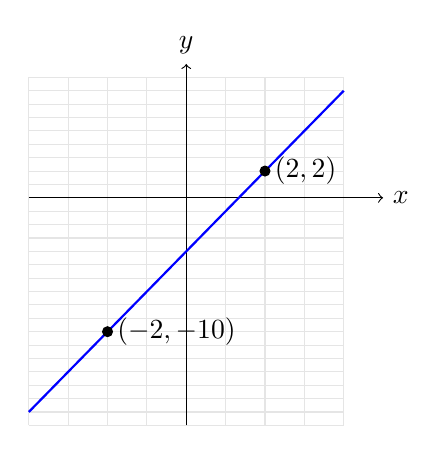
\begin{tikzpicture}[x=0.5cm,y=0.17cm]
\draw[step=1,gray!20] (-4,-17.0) grid (4,9.0);\draw[->] (-4,0)--(5,0) node[right] {$x$};\draw[->] (0,-17.0)--(0,10.0) node[above] {$y$};\draw[thick,blue] (-4,-16.0)--(4,8.0);\fill (-2,-10.0) circle (2pt);\node[right] at (-2,-10.0) {$(-2,-10)$};\fill (2,2.0) circle (2pt);\node[right] at (2,2.0) {$(2,2)$};
\end{tikzpicture}\end{center}
\textbf{Answer:} \(3\)
\textbf{Method:} Read two points and calculate rise/run.
\textbf{Reusable LaTeX template:}
\begin{verbatim}
Find the slope of the line in the graph.
\end{verbatim}
\textbf{Answer formula/rule:}
\begin{verbatim}
m
\end{verbatim}
\textbf{Generation ranges:} m: -3 to 3; b: -4 to 4
\textbf{Required extensions:} diagram\_renderer
\medskip\hrule\medskip
\subsection{F06 -- Interpret proportional slope}
\textbf{Targets:} A.5.c\quad\textbf{Mode:} numeric
\textbf{Question:} The distance-time equation is \(d=60t\), with miles and hours. What is the speed in miles per hour?
\textbf{Answer:} \(60\)
\textbf{Method:} The coefficient is distance per unit time.
\textbf{Reusable LaTeX template:}
\begin{verbatim}
The distance-time equation is \(d={r:10–80}t\), with miles and hours. What is the speed
in miles per hour?
\end{verbatim}
\textbf{Answer formula/rule:}
\begin{verbatim}
r
\end{verbatim}
\textbf{Generation ranges:} r: 10 to 80
\medskip\hrule\medskip
\subsection{F07 -- Graph a linear equation}
\textbf{Targets:} A.5.d\quad\textbf{Mode:} line\_graph
\textbf{Question:} Graph \(y=-2x+(-1)\).
\textbf{Answer:} \(y=-2x+(-1)\)
\textbf{Method:} Plot the y-intercept and another point using the slope.
\textbf{Reusable LaTeX template:}
\begin{verbatim}
Graph \(y={m:-4–4}x+({b:-6–6})\).
\end{verbatim}
\textbf{Answer formula/rule:}
\begin{verbatim}
y=m*x+b
\end{verbatim}
\textbf{Generation ranges:} m: -4 to 4; b: -6 to 6
\textbf{Required extensions:} line\_graph\_grading
\medskip\hrule\medskip
\subsection{F08 -- Linear y-intercept}
\textbf{Targets:} A.5.e\quad\textbf{Mode:} numeric
\textbf{Question:} A balance follows \(B(t)=7t+79\). Find the initial balance \(B(0)\).
\textbf{Answer:} \(79\)
\textbf{Method:} Evaluate at t=0; the intercept is the initial value.
\textbf{Reusable LaTeX template:}
\begin{verbatim}
A balance follows \(B(t)={m:1–20}t+{b:10–100}\). Find the initial balance \(B(0)\).
\end{verbatim}
\textbf{Answer formula/rule:}
\begin{verbatim}
b
\end{verbatim}
\textbf{Generation ranges:} m: 1 to 20; b: 10 to 100
\medskip\hrule\medskip
\subsection{F09 -- Linear x-intercept}
\textbf{Targets:} A.5.e\quad\textbf{Mode:} numeric
\textbf{Question:} Find the x-intercept coordinate of \(y=9x+(9)\). Enter only its x-coordinate.
\textbf{Answer:} \(-1\)
\textbf{Method:} Set y=0 and solve for x.
\textbf{Reusable LaTeX template:}
\begin{verbatim}
Find the x-intercept coordinate of \(y={m:1–10}x+({b:-20–20})\). Enter only its
x-coordinate.
\end{verbatim}
\textbf{Answer formula/rule:}
\begin{verbatim}
-b/m
\end{verbatim}
\textbf{Generation ranges:} m: 1 to 10; b: -20 to 20
\medskip\hrule\medskip
\subsection{F10 -- Quadratic vertex}
\textbf{Targets:} A.5.e\quad\textbf{Mode:} ordered\_pair
\textbf{Question:} Find the vertex of \(y=2(x-(-1))^2+(-10)\).
\textbf{Answer:} \((-1,-10)\)
\textbf{Method:} Vertex form gives vertex coordinates directly.
\textbf{Reusable LaTeX template:}
\begin{verbatim}
Find the vertex of \(y={a:1–5}(x-({h:-6–6}))^2+({k:-10–10})\).
\end{verbatim}
\textbf{Answer formula/rule:}
\begin{verbatim}
[h,k]
\end{verbatim}
\textbf{Generation ranges:} a: 1 to 5; h: -6 to 6; k: -10 to 10
\textbf{Required extensions:} ordered\_pair\_grading
\medskip\hrule\medskip
\subsection{F11 -- Quadratic minimum}
\textbf{Targets:} A.5.e\quad\textbf{Mode:} numeric
\textbf{Question:} Find the minimum value of \(y=3(x-(-5))^2+(10)\).
\textbf{Answer:} \(10\)
\textbf{Method:} A positive squared-term coefficient gives minimum k.
\textbf{Reusable LaTeX template:}
\begin{verbatim}
Find the minimum value of \(y={a:1–5}(x-({h:-6–6}))^2+({k:-10–10})\).
\end{verbatim}
\textbf{Answer formula/rule:}
\begin{verbatim}
k
\end{verbatim}
\textbf{Generation ranges:} a: 1 to 5; h: -6 to 6; k: -10 to 10
\medskip\hrule\medskip
\subsection{F12 -- Quadratic symmetry axis}
\textbf{Targets:} A.5.e\quad\textbf{Mode:} numeric
\textbf{Question:} Find the axis of symmetry of \(y=3(x-(4))^2+(3)\). Enter the x-value of the axis.
\textbf{Answer:} \(4\)
\textbf{Method:} The symmetry axis passes through the vertex.
\textbf{Reusable LaTeX template:}
\begin{verbatim}
Find the axis of symmetry of \(y={a:1–5}(x-({h:-6–6}))^2+({k:-10–10})\). Enter the
x-value of the axis.
\end{verbatim}
\textbf{Answer formula/rule:}
\begin{verbatim}
h
\end{verbatim}
\textbf{Generation ranges:} a: 1 to 5; h: -6 to 6; k: -10 to 10
\medskip\hrule\medskip
\subsection{F13 -- Increasing interval of a quadratic}
\textbf{Targets:} A.5.e\quad\textbf{Mode:} interval
\textbf{Question:} For \(y=(x-(-3))^2+-8\), give the open interval where the function is increasing.
\textbf{Answer:} \((-3,\infty)\)
\textbf{Method:} The upward-opening parabola increases to the right of its vertex.
\textbf{Reusable LaTeX template:}
\begin{verbatim}
For \(y=(x-({h:-6–6}))^2+{k:-10–10}\), give the open interval where the function is
increasing.
\end{verbatim}
\textbf{Answer formula/rule:}
\begin{verbatim}
(h,infinity)
\end{verbatim}
\textbf{Generation ranges:} h: -6 to 6; k: -10 to 10
\textbf{Required extensions:} interval\_grading
\medskip\hrule\medskip
\subsection{F14 -- Line through slope and point}
\textbf{Targets:} A.6.a\quad\textbf{Mode:} equation
\textbf{Question:} Write an equation for the line with slope 5 through \((0,5)\).
\textbf{Answer:} \(y=5(x-(0))+(5)\)
\textbf{Method:} Use point-slope form; equivalent line equations are accepted.
\textbf{Reusable LaTeX template:}
\begin{verbatim}
Write an equation for the line with slope {m:-6–6} through \(({a:-6–6},{b:-10–10})\).
\end{verbatim}
\textbf{Answer formula/rule:}
\begin{verbatim}
y=m*(x-a)+b
\end{verbatim}
\textbf{Generation ranges:} m: -6 to 6; a: -6 to 6; b: -10 to 10
\textbf{Required extensions:} equation\_grading
\medskip\hrule\medskip
\subsection{F15 -- Line through two points}
\textbf{Targets:} A.6.b\quad\textbf{Mode:} equation
\textbf{Question:} Write an equation for the line through \((-5,-5)\) and \((0,15)\).
\textbf{Answer:} \(y=4(x-(-5))+(-5)\)
\textbf{Method:} Find the slope, then use point-slope form; symbols x0,y0 are stored point values.
\textbf{Reusable LaTeX template:}
\begin{verbatim}
Write an equation for the line through \(({x0:-5–5},{y0:-10–10})\) and \(({u},{v})\).
\end{verbatim}
\textbf{Answer formula/rule:}
\begin{verbatim}
y=((v-y0)/(u-x0))*(x-x0)+y0
\end{verbatim}
\textbf{Generation ranges:} x0: -5 to 5; y0: -10 to 10; dx: 1 to 6; m: -5 to 5
\textbf{Derived variables:} u = x0+dx; v = y0+m*dx
\textbf{Required extensions:} derived\_variables, equation\_grading
\medskip\hrule\medskip
\subsection{F16 -- Parallel line slope}
\textbf{Targets:} A.6.c\quad\textbf{Mode:} numeric
\textbf{Question:} A line has slope -4. Find the slope of any distinct parallel line.
\textbf{Answer:} \(-4\)
\textbf{Method:} Nonvertical parallel lines have equal slopes.
\textbf{Reusable LaTeX template:}
\begin{verbatim}
A line has slope {m:-8–8}. Find the slope of any distinct parallel line.
\end{verbatim}
\textbf{Answer formula/rule:}
\begin{verbatim}
m
\end{verbatim}
\textbf{Generation ranges:} m: -8 to 8
\medskip\hrule\medskip
\subsection{F17 -- Perpendicular line slope}
\textbf{Targets:} A.6.c\quad\textbf{Mode:} numeric
\textbf{Question:} A line has nonzero slope 9. Find the slope of a perpendicular line.
\textbf{Answer:} \(\frac{-1}{9}\)
\textbf{Method:} Use the negative reciprocal.
\textbf{Reusable LaTeX template:}
\begin{verbatim}
A line has nonzero slope {m:1–10}. Find the slope of a perpendicular line.
\end{verbatim}
\textbf{Answer formula/rule:}
\begin{verbatim}
-1/m
\end{verbatim}
\textbf{Generation ranges:} m: 1 to 10
\medskip\hrule\medskip
\subsection{F18 -- Compare proportional speeds}
\textbf{Targets:} A.7.a\quad\textbf{Mode:} category
\textbf{Question:} Car A travels 155 miles in 3 hours at constant speed. Car B obeys \(d_B=72t_B\). Which car is faster: A, B, or equal?
\textbf{Answer:} \(\text{B}\)
\textbf{Method:} Compare A speed d/t with B slope r.
\textbf{Reusable LaTeX template:}
\begin{verbatim}
Car A travels {d:30–180} miles in {t:1–4} hours at constant speed. Car B obeys
\(d_B={r:10–80}t_B\). Which car is faster: A, B, or equal?
\end{verbatim}
\textbf{Answer formula/rule:}
\begin{verbatim}
compare(d/t,r)
\end{verbatim}
\textbf{Generation ranges:} d: 30 to 180; t: 1 to 4; r: 10 to 80
\textbf{Required extensions:} category\_grading
\medskip\hrule\medskip
\subsection{F19 -- Identify a function from a table}
\textbf{Targets:} A.7.b\quad\textbf{Mode:} category
\textbf{Question:} Does this table define y as a function of x? Answer yes or no. \(\begin{array}{c|ccc}x&5&5&8\\y&4&6&3\end{array}\)
\textbf{Answer:} \(\text{no}\)
\textbf{Method:} The input a has two different outputs, u and v.
\textbf{Reusable LaTeX template:}
\begin{verbatim}
Does this table define y as a function of x? Answer yes or no.
\(\begin{array}{c|ccc}x&{a:1–5}&{a}&{b}\\y&{u:1–10}&{v}&{w:1–10}\end{array}\)
\end{verbatim}
\textbf{Answer formula/rule:}
\begin{verbatim}
no
\end{verbatim}
\textbf{Generation ranges:} a: 1 to 5; k: 1 to 5; u: 1 to 10; j: 1 to 5; w: 1 to 10
\textbf{Derived variables:} b = a+k; v = u+j
\textbf{Required extensions:} derived\_variables, category\_grading
\medskip\hrule\medskip
\subsection{F20 -- Evaluate a linear function}
\textbf{Targets:} A.7.c\quad\textbf{Mode:} numeric
\textbf{Question:} If \(f(x)=5x+(6)\), find \(f(9)\).
\textbf{Answer:} \(51\)
\textbf{Method:} Substitute v for x.
\textbf{Reusable LaTeX template:}
\begin{verbatim}
If \(f(x)={a:-8–8}x+({b:-15–15})\), find \(f({v:-10–10})\).
\end{verbatim}
\textbf{Answer formula/rule:}
\begin{verbatim}
a*v+b
\end{verbatim}
\textbf{Generation ranges:} a: -8 to 8; b: -15 to 15; v: -10 to 10
\medskip\hrule\medskip
\subsection{F21 -- Evaluate a quadratic function}
\textbf{Targets:} A.7.c\quad\textbf{Mode:} numeric
\textbf{Question:} If \(f(x)=5x^2+(-5)x+(-15)\), find \(f(-4)\).
\textbf{Answer:} \(85\)
\textbf{Method:} Substitute the input and evaluate the polynomial.
\textbf{Reusable LaTeX template:}
\begin{verbatim}
If \(f(x)={a:1–5}x^2+({b:-10–10})x+({c:-15–15})\), find \(f({v:-6–6})\).
\end{verbatim}
\textbf{Answer formula/rule:}
\begin{verbatim}
a*v*v+b*v+c
\end{verbatim}
\textbf{Generation ranges:} a: 1 to 5; b: -10 to 10; c: -15 to 15; v: -6 to 6
\medskip\hrule\medskip
\subsection{F22 -- Compare rates from table and equation}
\textbf{Targets:} A.7.d\quad\textbf{Mode:} category
\textbf{Question:} Function A is \(y=-3x+-1\). Function B has table \(\begin{array}{c|cc}x&0&2\\y&-5&-5\end{array}\). Which has the greater slope: A, B, or equal?
\textbf{Answer:} \(\text{B}\)
\textbf{Method:} Compare r with the table rate (v-u)/d.
\textbf{Reusable LaTeX template:}
\begin{verbatim}
Function A is \(y={r:-6–6}x+{c:-10–10}\). Function B has table
\(\begin{array}{c|cc}x&0&{d:1–5}\\y&{u:-10–10}&{v}\end{array}\). Which has the greater
slope: A, B, or equal?
\end{verbatim}
\textbf{Answer formula/rule:}
\begin{verbatim}
compare(r,(v-u)/d)
\end{verbatim}
\textbf{Generation ranges:} r: -6 to 6; c: -10 to 10; d: 1 to 5; u: -10 to 10; m: -6 to 6
\textbf{Derived variables:} v = u+m*d
\textbf{Required extensions:} derived\_variables, category\_grading
\medskip\hrule\medskip
\end{document}
